\documentclass[11pt,a4paper]{article}

\usepackage[T1]{fontenc}
\usepackage[utf8]{inputenc}
\usepackage[english]{babel}
\usepackage[a4paper,margin=0.62in]{geometry}
\usepackage{parskip}
\usepackage{graphicx}
\usepackage{booktabs}
\usepackage{tabularx}
\usepackage{longtable}
\usepackage{float}
\usepackage{xcolor}
\usepackage[colorlinks=true,linkcolor=blue!55!black,urlcolor=blue!55!black]{hyperref}

\linespread{1.0}
\setlength{\parskip}{0.5em}
\setlength{\parindent}{0pt}
\emergencystretch=1.5em
\pagestyle{plain}

\newcommand{\figref}[1]{\hyperref[#1]{Figure~\ref*{#1}}}
\newcommand{\appendixfig}[2]{%
  \noindent\includegraphics[width=\columnwidth]{#1}\\[-0.2em]
  {\footnotesize \textbf{#2}.}%
  \par\vspace{0.85em}
}

\title{\textbf{DSA210 Term Project: Data Collection, EDA, and Hypothesis Testing}}
\author{
Nihat Ömer Karaca\\
Student ID: 30626\\
\texttt{omer.karaca@sabanciuniv.edu}\\
\texttt{nihatomer.karaca@gmail.com}
}
\date{}

\begin{document}
\maketitle
\vspace{-1.1em}

\section*{Introduction}
This project studies how my entertainment behavior changes under academic pressure. The original motivation was practical: during ordinary weeks, midterms, and finals, I felt that my use of entertainment platforms might not stay the same. Instead of keeping this as an intuition, I collected and prepared my own platform exports so that I could test the idea with data.

At first, I considered several personal data exports, including ChatGPT, Instagram, Netflix, Spotify, Twitter, and YouTube. After checking the scope and privacy risks, I decided to postpone ChatGPT because it is a different domain and would require heavier privacy and text-processing decisions. I also excluded Instagram and Twitter from this stage because they would increase the complexity of the project more than they would improve the current analysis. Therefore, the current version focuses on YouTube, Spotify, Netflix, Prime Video, and the academic calendar.

The final structure is intentionally entertainment-focused. YouTube represents short-form and mixed video behavior, Spotify represents music listening duration, and Netflix plus Prime Video represent long-form streaming. The academic calendar is not treated as a behavioral dataset; instead, it is used as a label source so that ordinary term days and final-exam days can be compared.

\section*{Data Collection and Preparation}
The public prepared datasets are stored under \texttt{data\_github/}. The private raw exports were not equally clean. Spotify was already structured, YouTube needed activity normalization and masking, Netflix was simple but only date-level, and Prime Video required parsing into movie and episode records. Because of these differences, the platform scripts first converted each source into a processed row-level table, then created shared \texttt{fine\_*} fields, and finally created public tables with private identifiers and local source paths removed.

\begin{table}[H]
\centering
\small
\caption{Prepared public datasets used in the current analysis.}
\label{tab:datasets}
\begin{tabularx}{\textwidth}{l r l X}
\toprule
\textbf{Dataset} & \textbf{Rows} & \textbf{Date range} & \textbf{Role in analysis}\\
\midrule
YouTube & 34,317 activity rows & 2022-04-17 to 2026-03-15 & Watch/search-style video activity with timestamps.\\
Spotify & 178,202 streaming rows & 2019-07-27 to 2026-03-14 & Music listening with timestamps and duration.\\
Netflix & 2,493 viewing rows & 2020-02-25 to 2026-03-10 & Long-form viewing history with visible titles.\\
Prime Video & 719 watch rows & 2022-03-30 to 2026-03-19 & Long-form viewing parsed into movie and episode records.\\
Academic calendar & 15 calendar rows & 2021--2022 to 2025--2026 & Period labels for ordinary term and final-exam days.\\
\bottomrule
\end{tabularx}
\end{table}

The common comparison window is from 2022-04-17 to 2026-03-10. This window was selected because all four behavioral datasets have data inside this range. After aggregation, the combined panel contains 1,424 daily rows. If a platform had no row on a date, that platform was treated as zero activity for that date after daily aggregation. This creates a common ground for testing across platforms without pretending that all raw exports measure the same thing.

\section*{Exploratory Data Analysis}
The EDA was done in two layers. First, I inspected each dataset separately to understand its structure, missingness, timing, and platform-specific behavior. Second, I created a combined daily EDA layer where YouTube, Spotify, Netflix, Prime Video, and the academic calendar labels were examined together. The most important figures are included in the main report, and the remaining EDA figures are embedded in the appendix.

\subsection*{Individual Platform EDA}
The YouTube EDA showed that the dataset is mainly watch activity, with search activity as a smaller secondary behavior. \figref{fig:youtube-actions} shows the action split, and \figref{fig:youtube-monthly} shows that watched and search counts are not stable over time.

\begin{figure}[H]
\centering
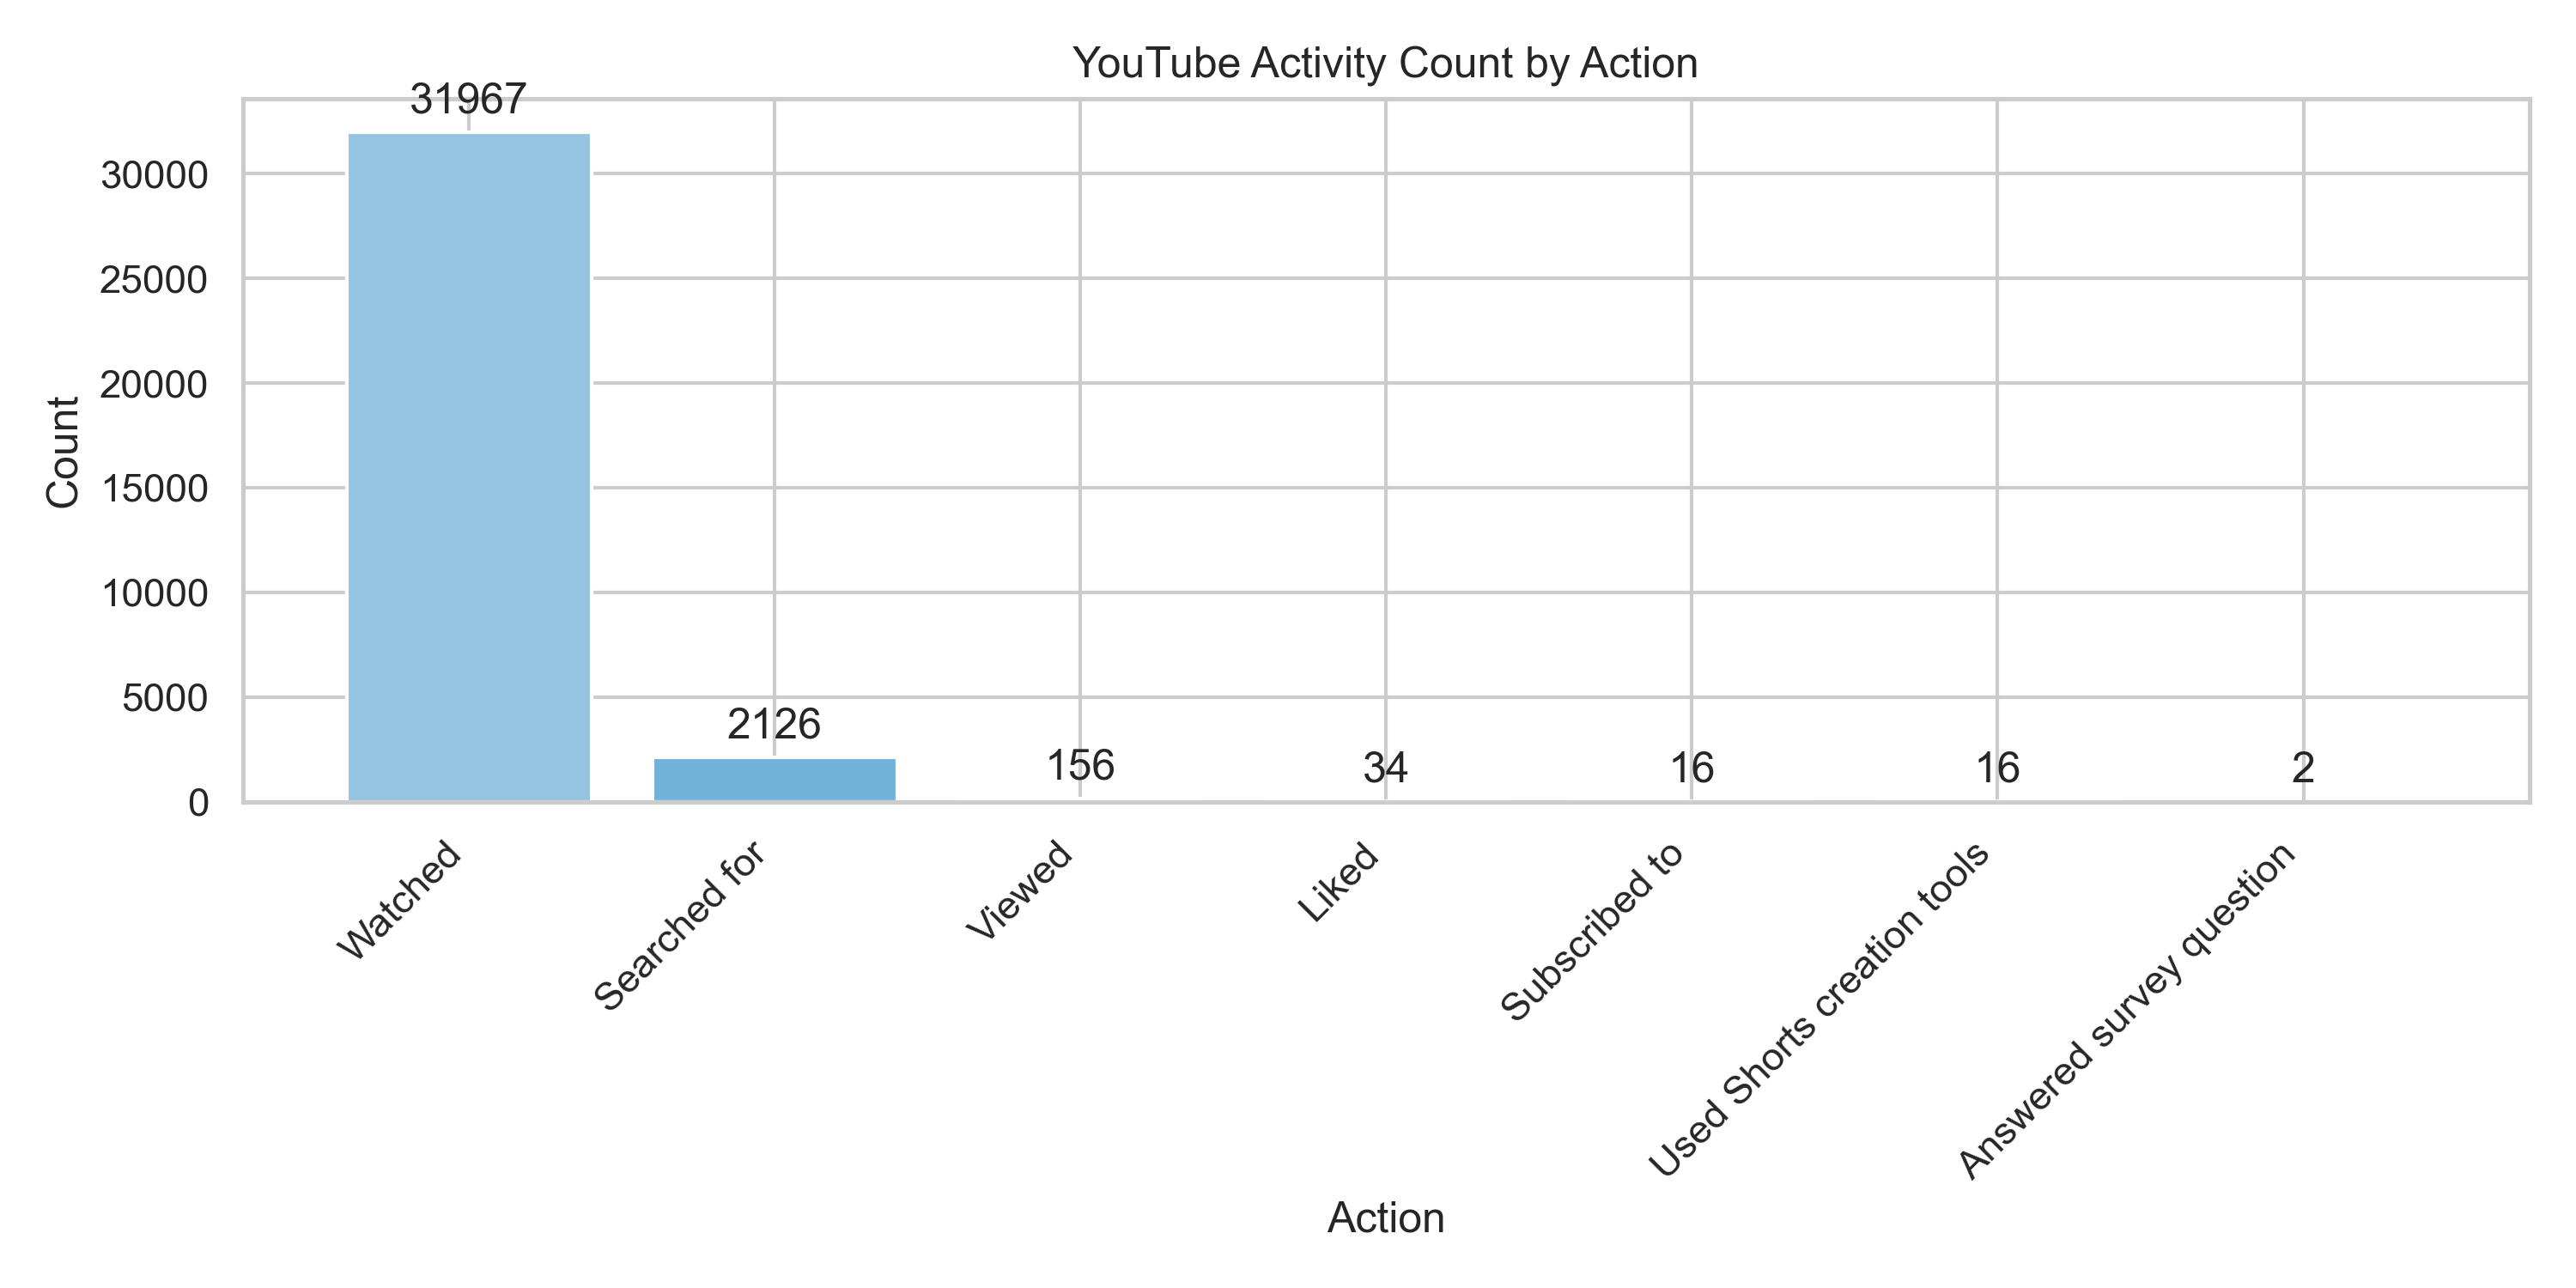
\includegraphics[width=0.86\textwidth]{../EDA/youtube_images/youtube_activity_count_by_action.png}
\caption{YouTube activity by action. This figure checks what kind of YouTube rows dominate the dataset.}
\label{fig:youtube-actions}
\end{figure}

\begin{figure}[H]
\centering
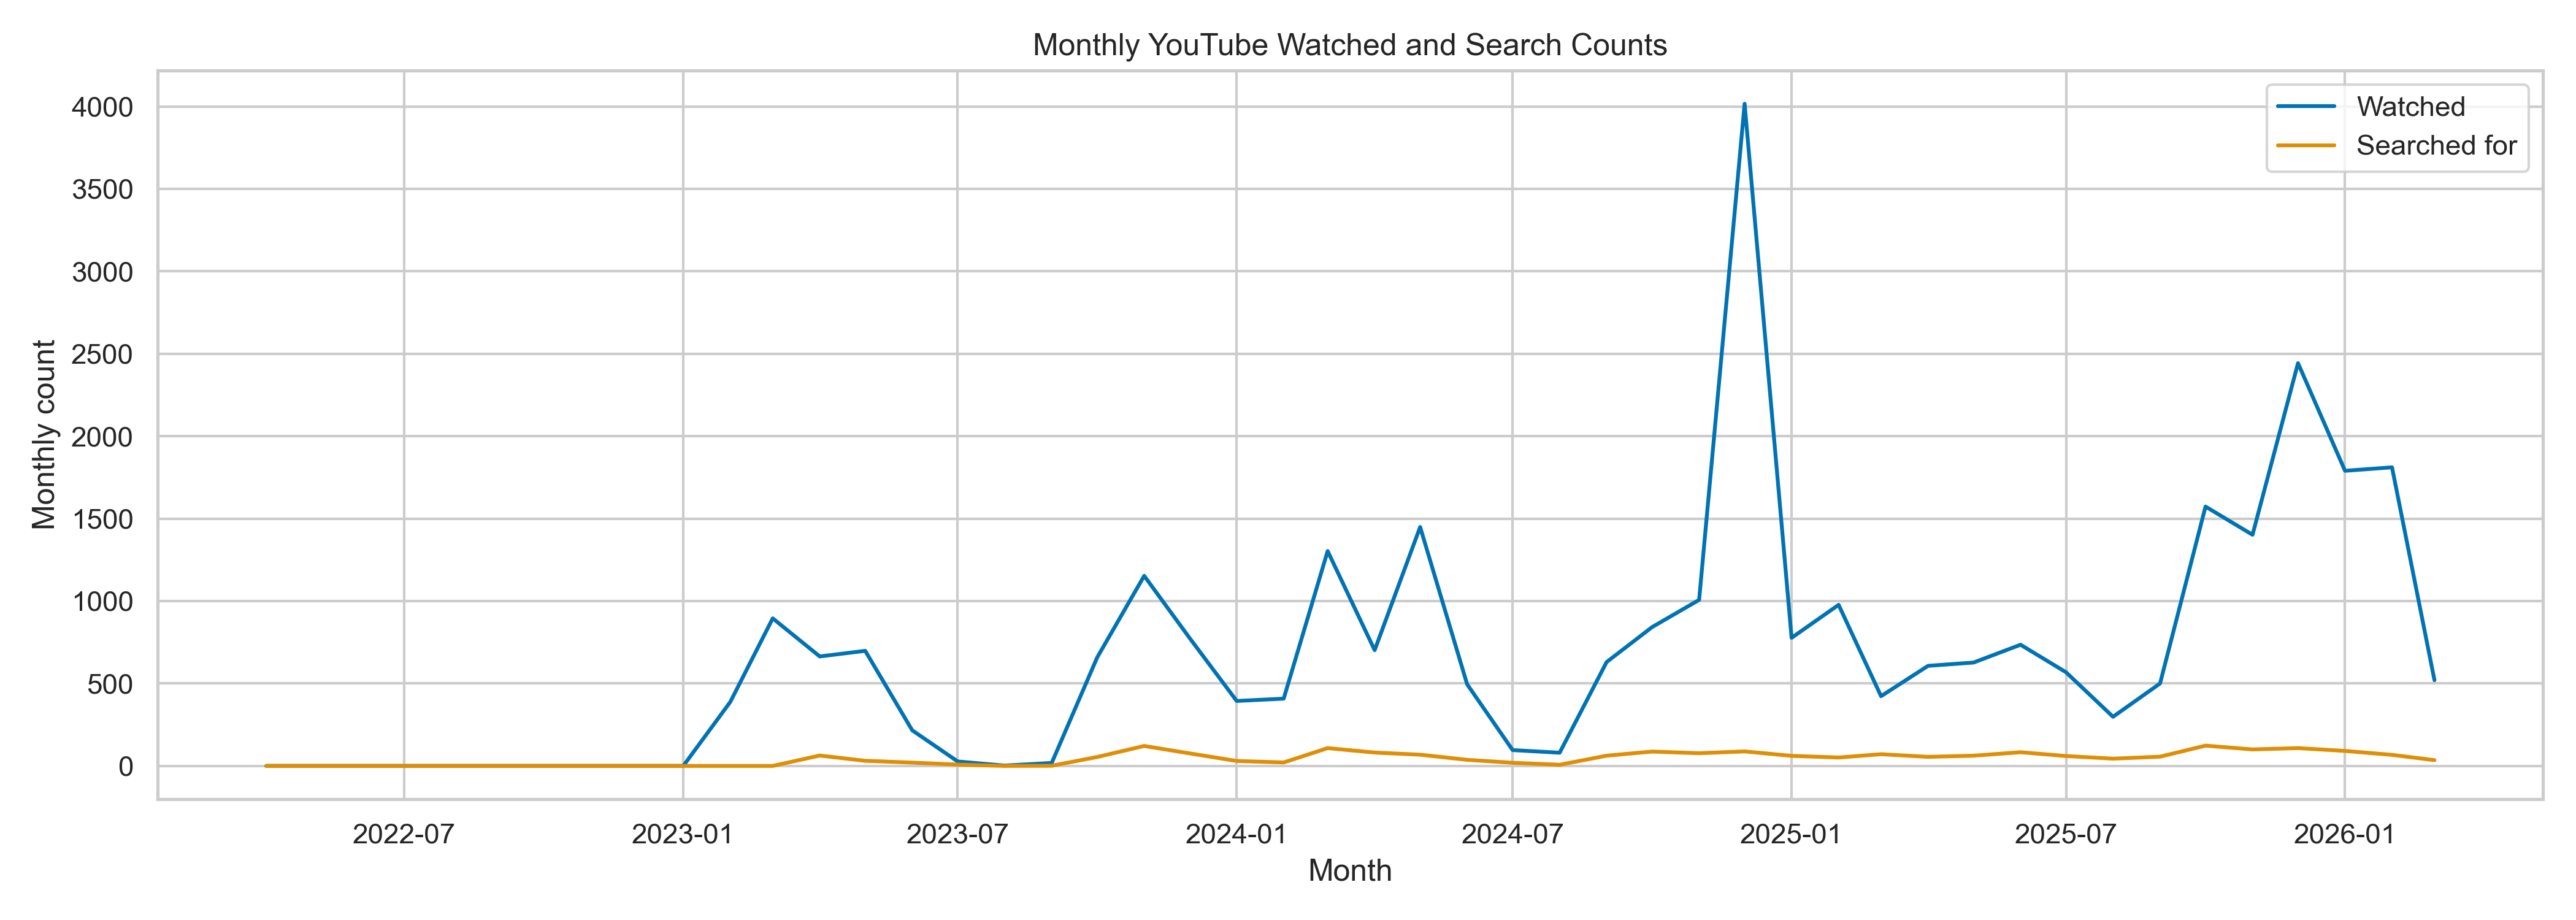
\includegraphics[width=0.86\textwidth]{../EDA/youtube_images/youtube_monthly_watched_and_search_counts.png}
\caption{Monthly YouTube watched and search counts. This figure gives a first view of the time trend in YouTube activity.}
\label{fig:youtube-monthly}
\end{figure}

The Spotify EDA was more duration-focused because Spotify provides listening time. \figref{fig:spotify-monthly} shows the monthly listening hours, while \figref{fig:spotify-streams-hours} checks the relationship between daily stream count and daily listening hours.

\begin{figure}[H]
\centering
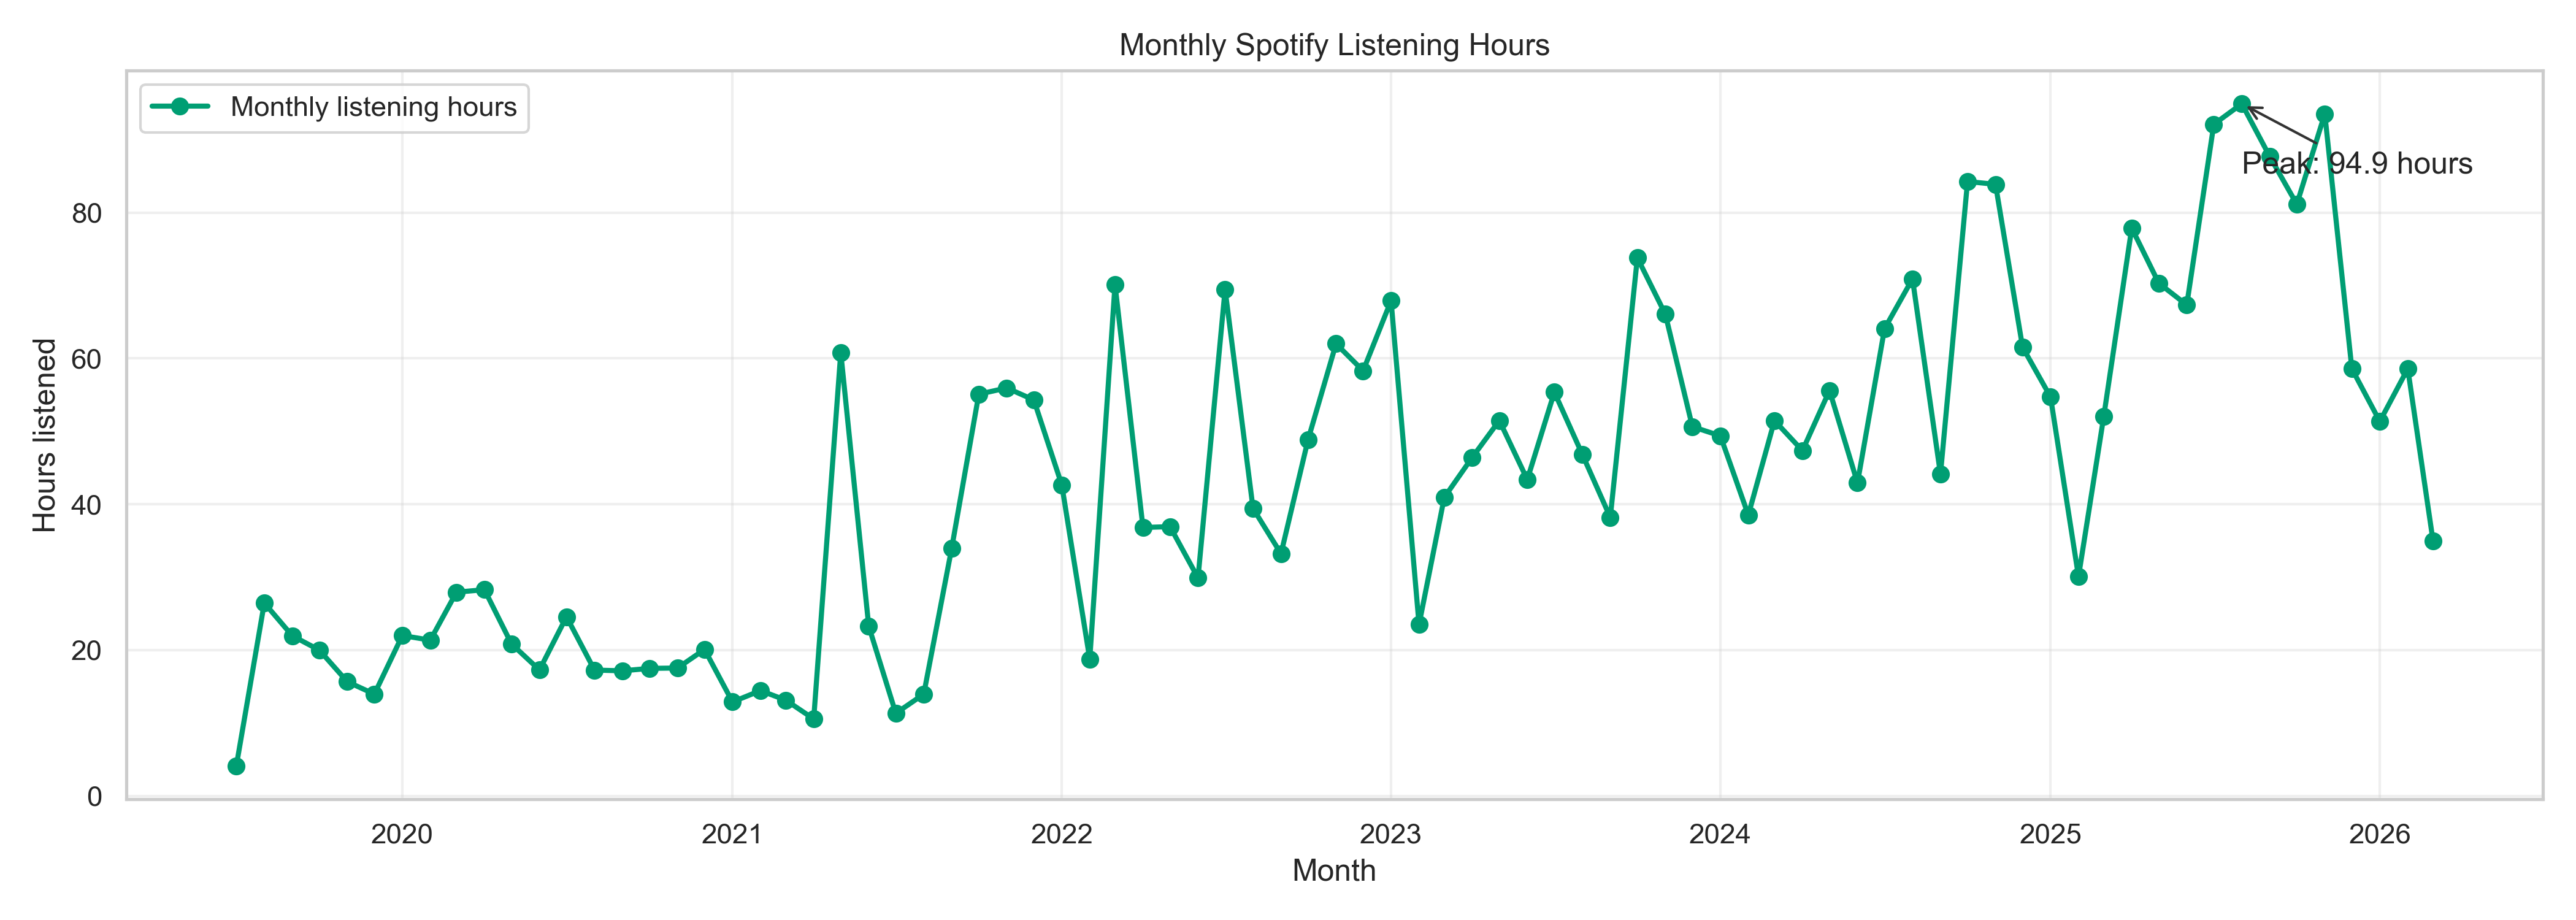
\includegraphics[width=0.86\textwidth]{../EDA/spotify_images/spotify_monthly_listening_hours.png}
\caption{Monthly Spotify listening hours. This shows how music listening changes over time.}
\label{fig:spotify-monthly}
\end{figure}

\begin{figure}[H]
\centering
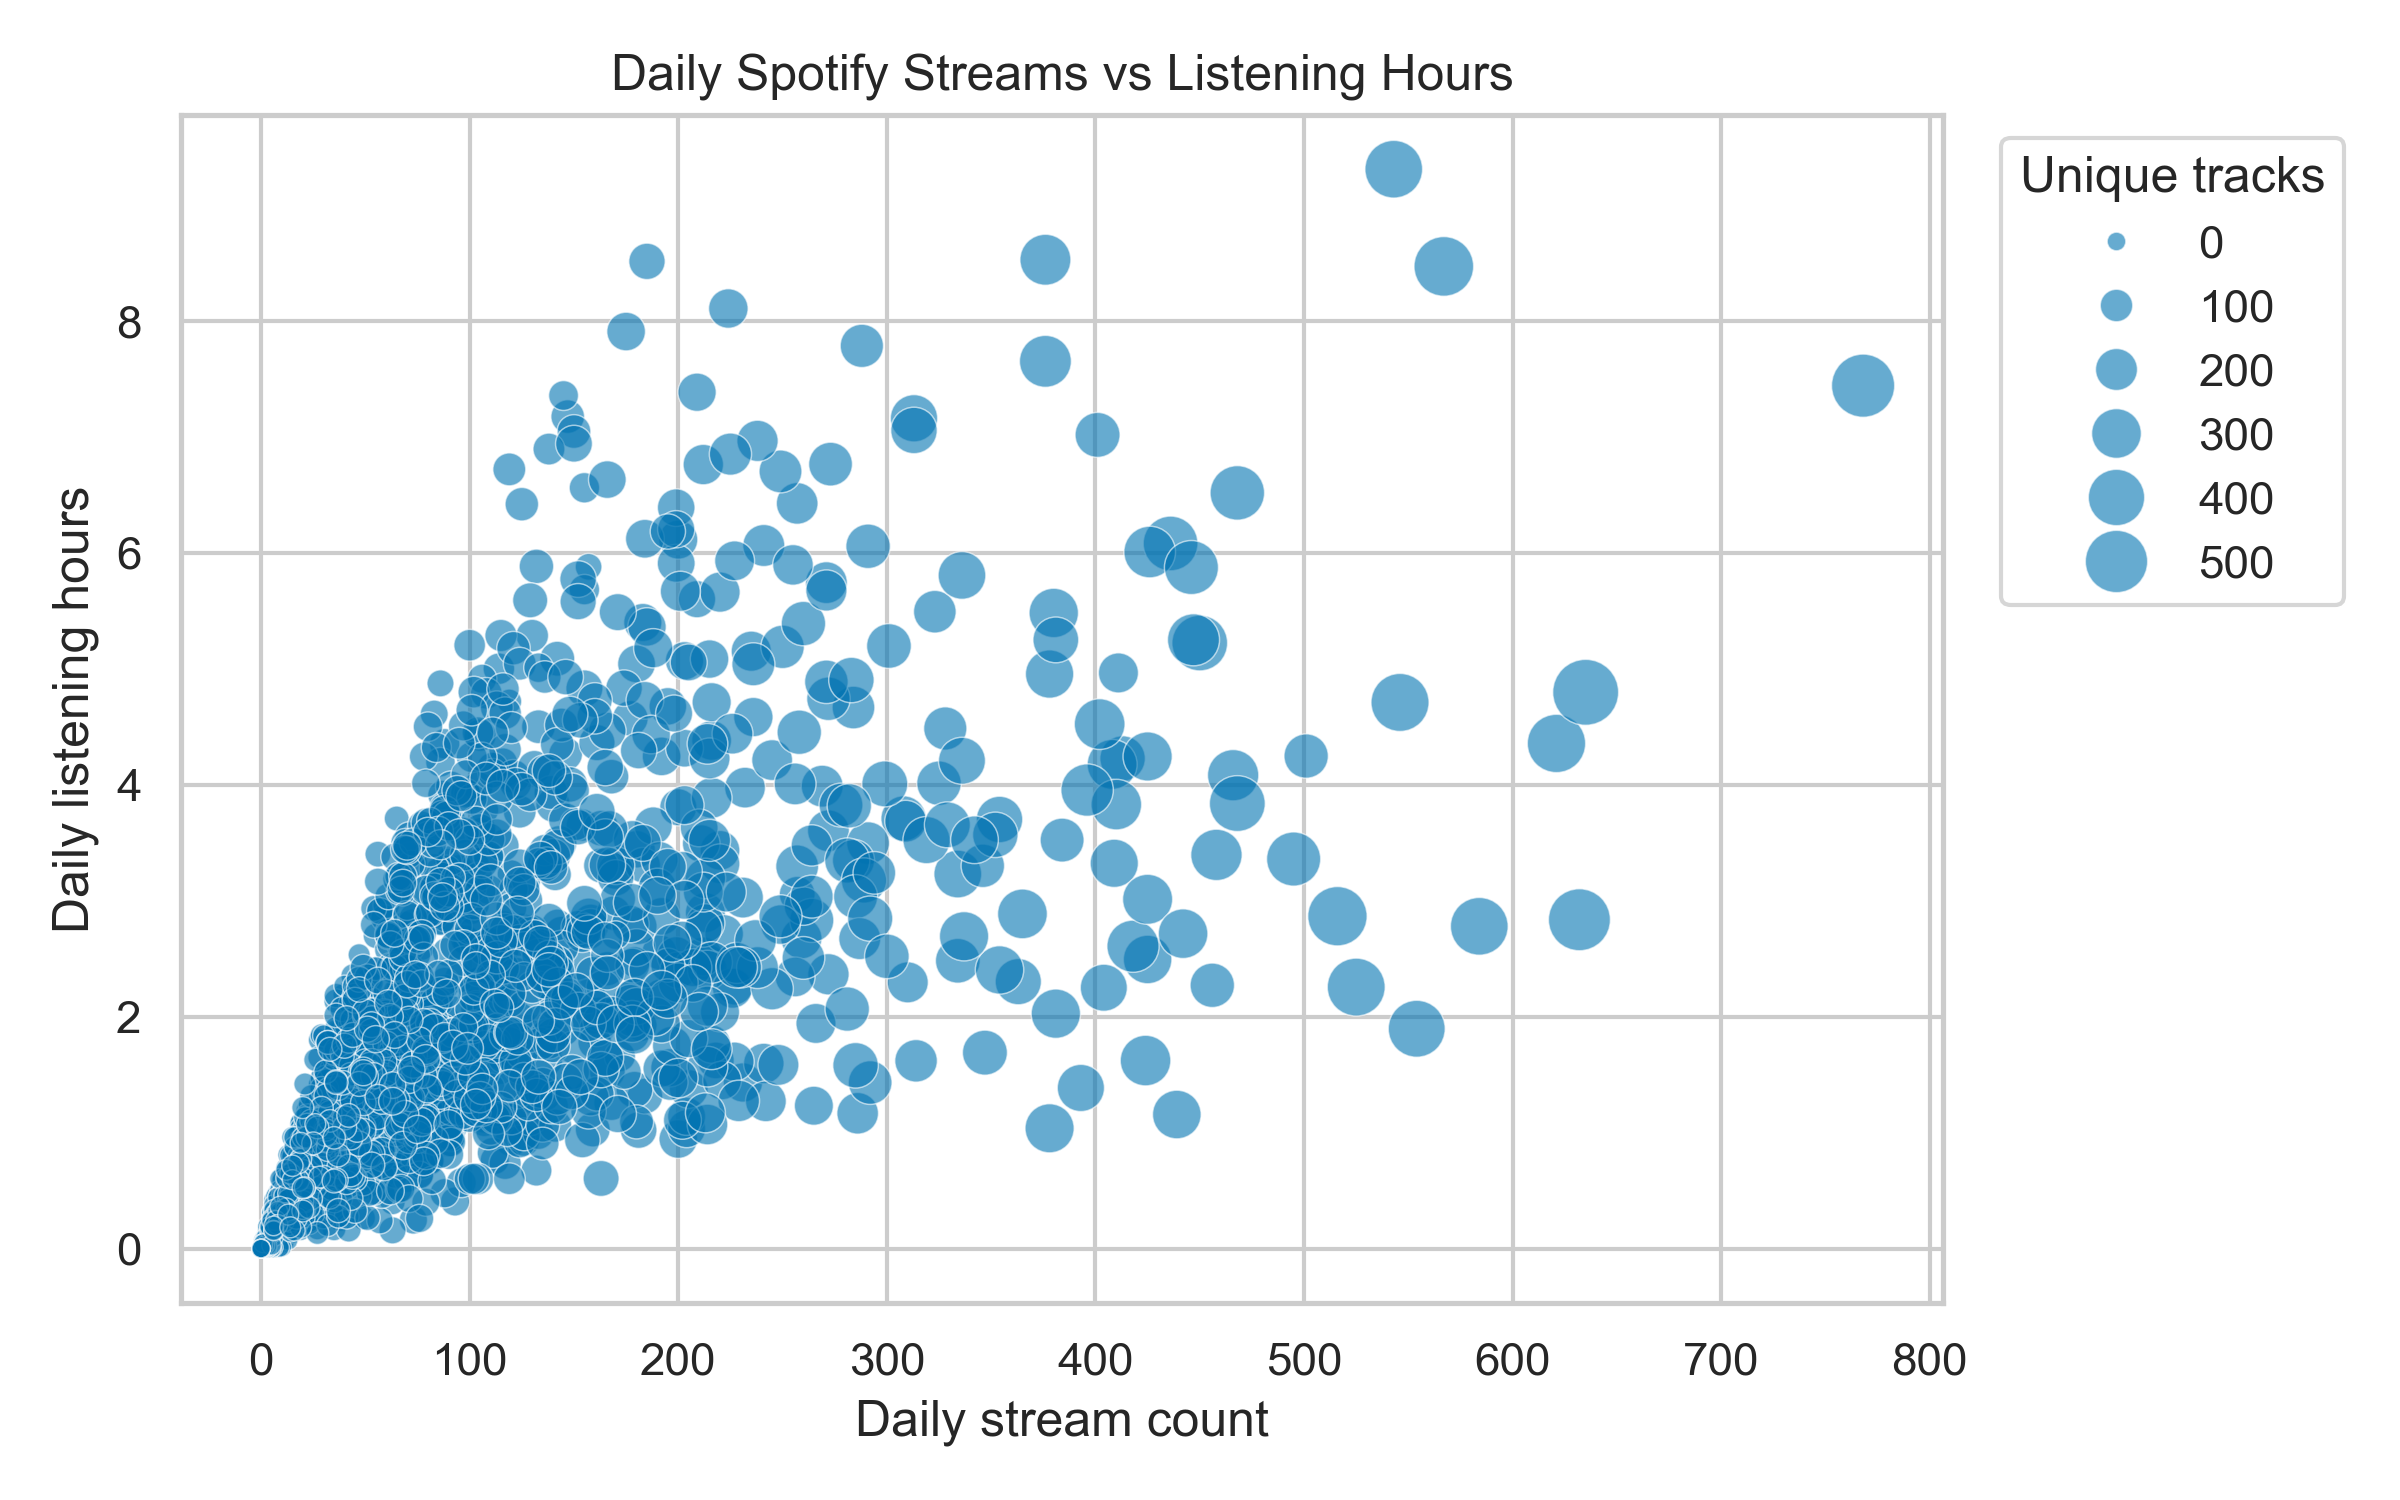
\includegraphics[width=0.86\textwidth]{../EDA/spotify_images/spotify_daily_streams_vs_hours.png}
\caption{Daily Spotify streams versus listening hours. This checks whether stream count and duration move together.}
\label{fig:spotify-streams-hours}
\end{figure}

Netflix and Prime Video were kept as separate public datasets, but in the EDA layer they were also grouped as long-form streaming. This was done because both platforms represent watching episodes or movies, while their raw exports are not identical. \figref{fig:longform-platform} compares their total counts, and \figref{fig:longform-monthly} shows the combined long-form trend.

\begin{figure}[H]
\centering
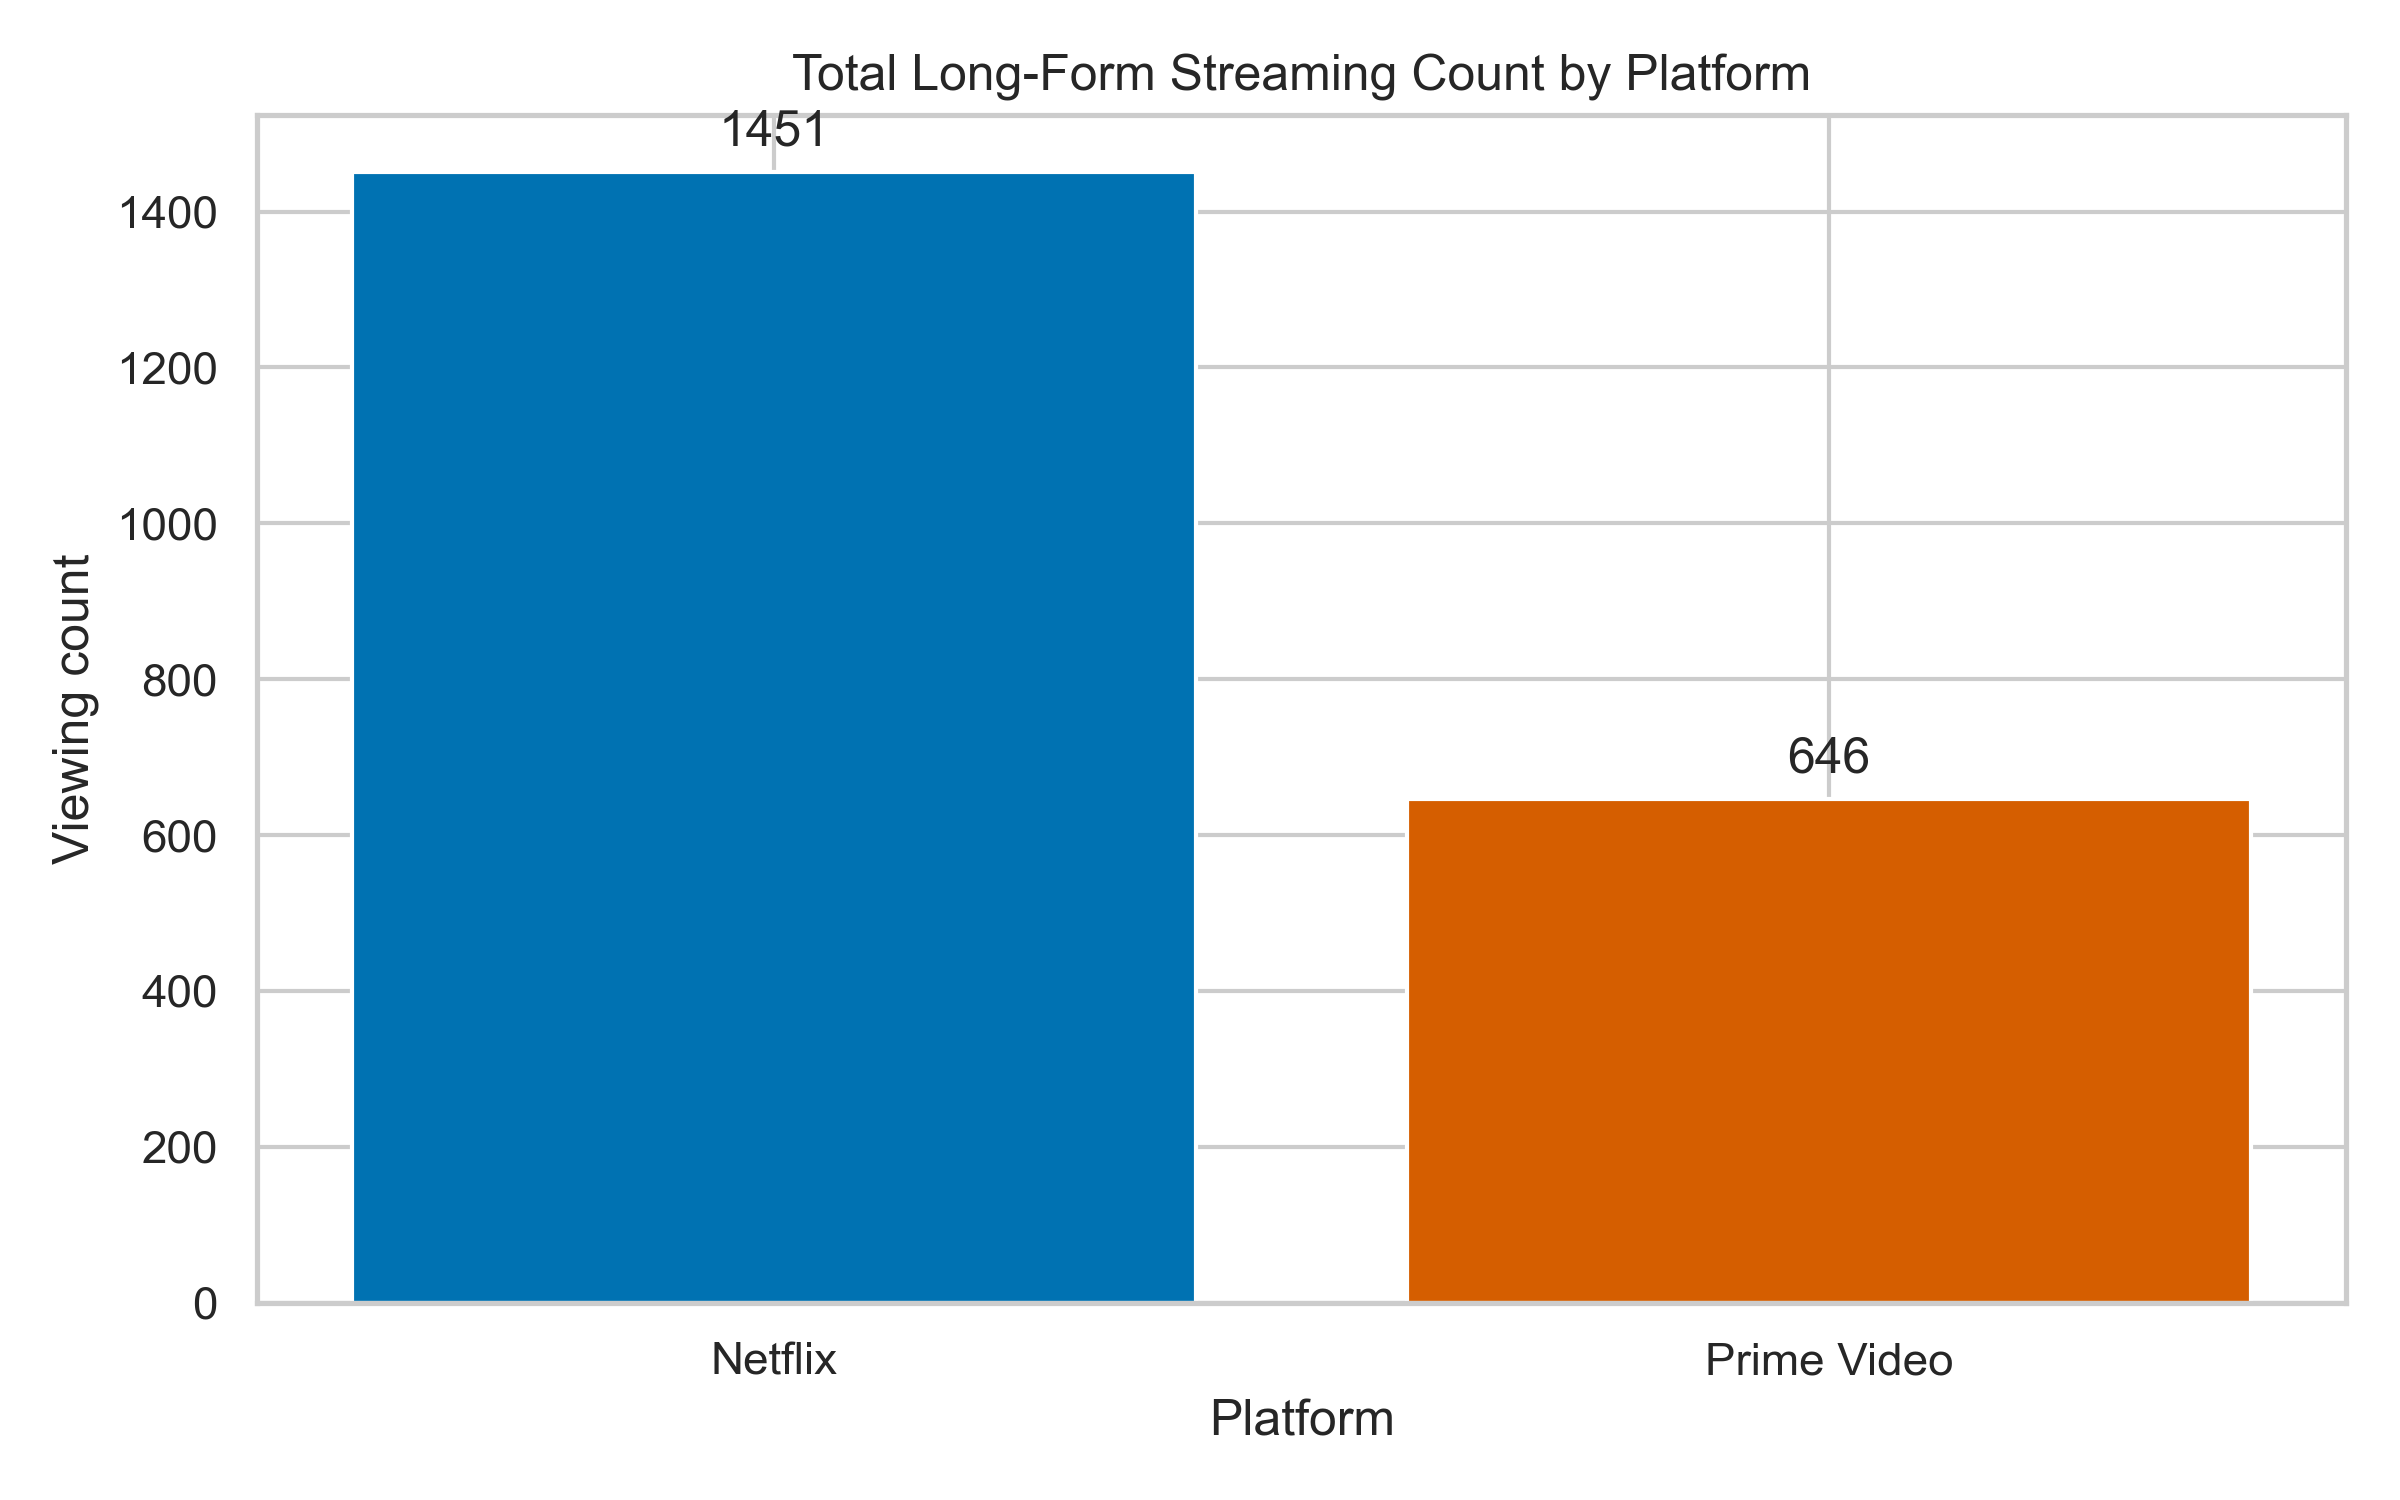
\includegraphics[width=0.86\textwidth]{../EDA/prime_netflix_images/total_long_form_count_by_platform_common_range.png}
\caption{Total long-form count by platform in the common comparison range. This shows the relative contribution of Netflix and Prime Video.}
\label{fig:longform-platform}
\end{figure}

\begin{figure}[H]
\centering
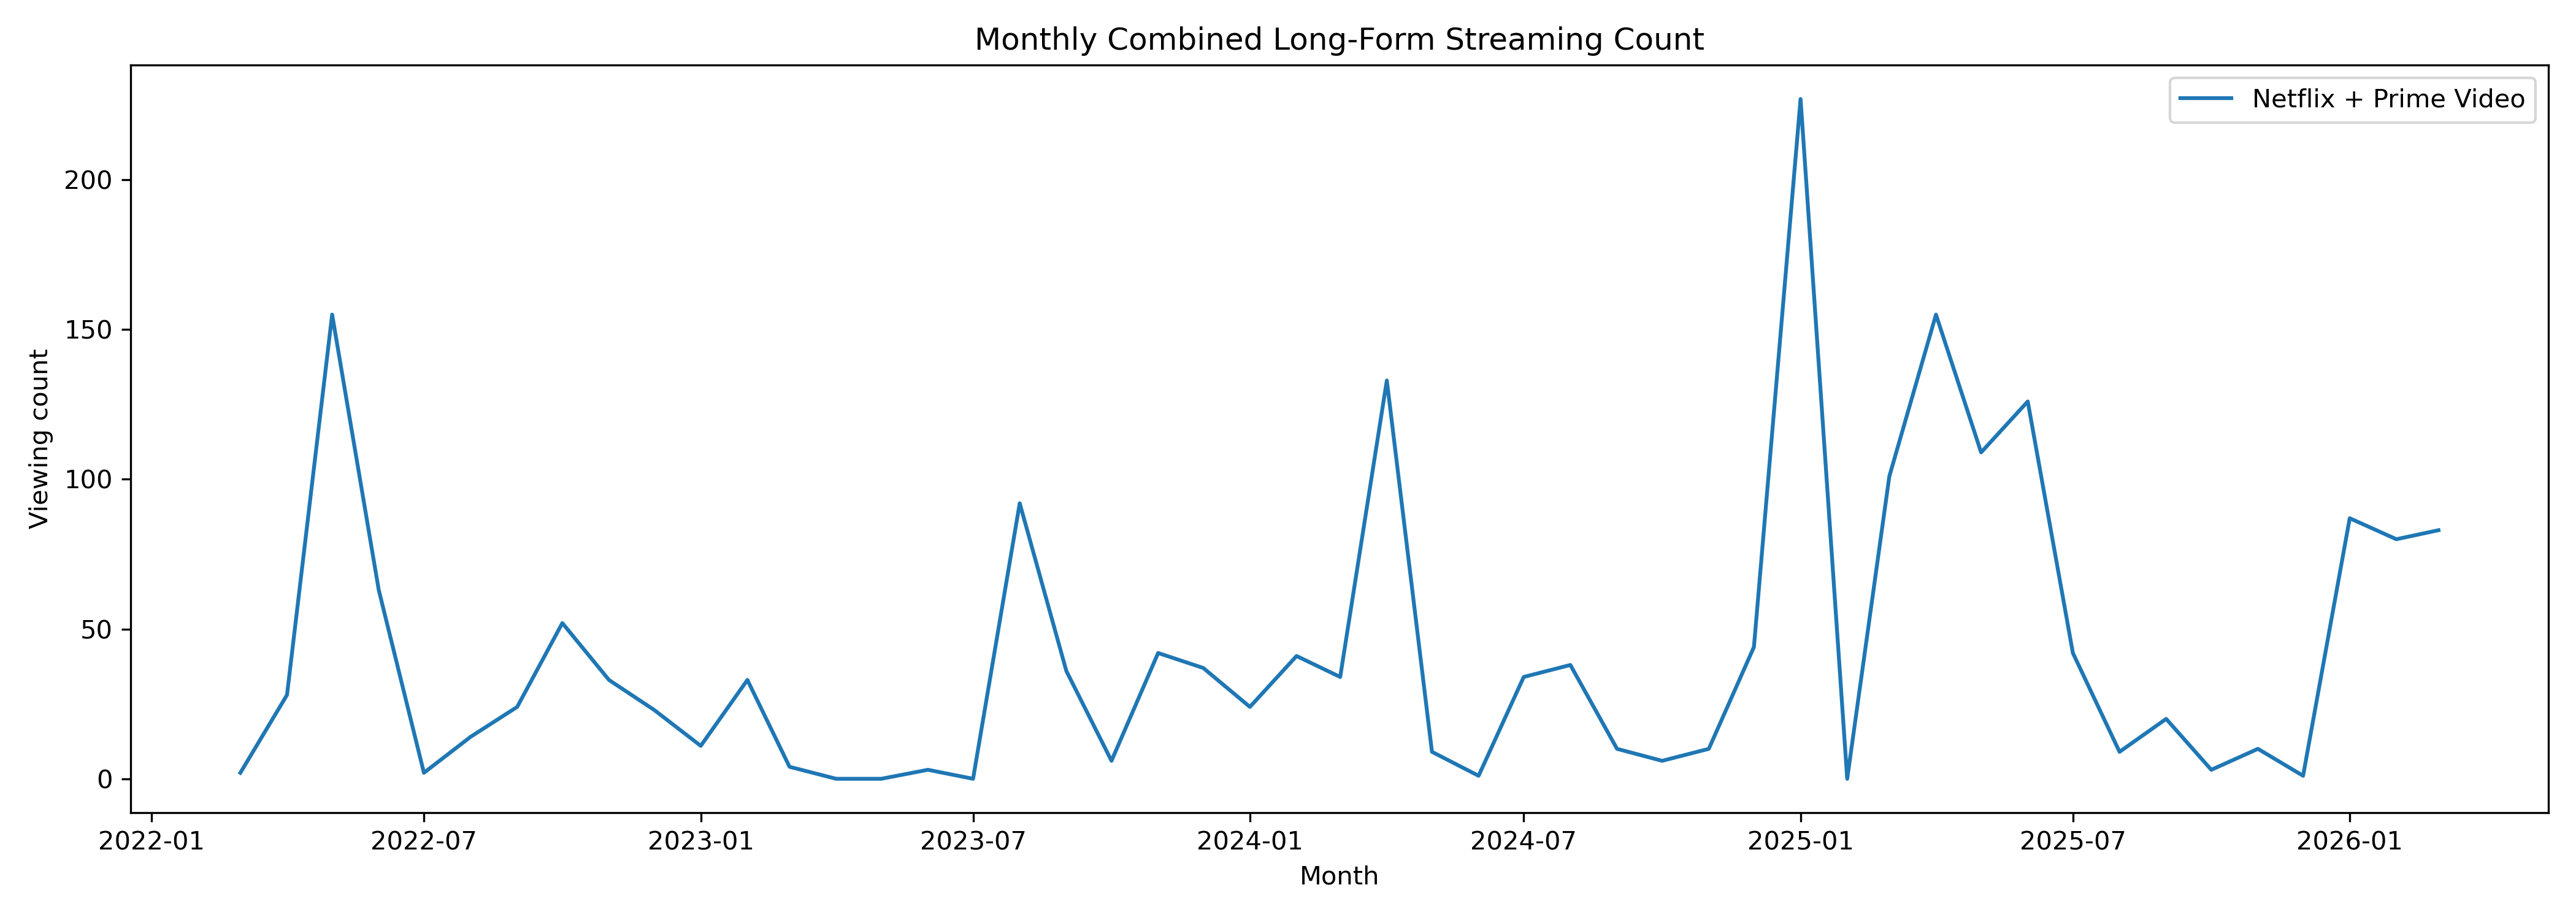
\includegraphics[width=0.86\textwidth]{../EDA/prime_netflix_images/monthly_combined_long_form_count.png}
\caption{Monthly combined long-form streaming count. This shows the bursty behavior of Netflix plus Prime Video.}
\label{fig:longform-monthly}
\end{figure}

\subsection*{Combined EDA}
The combined EDA was needed before testing the hypotheses. \figref{fig:coverage} shows the common comparison window, and \figref{fig:active-days} shows that the platforms do not have the same activity density. Spotify is much more continuous than Netflix or Prime Video, so raw cross-platform comparisons must be interpreted carefully.

\begin{figure}[H]
\centering
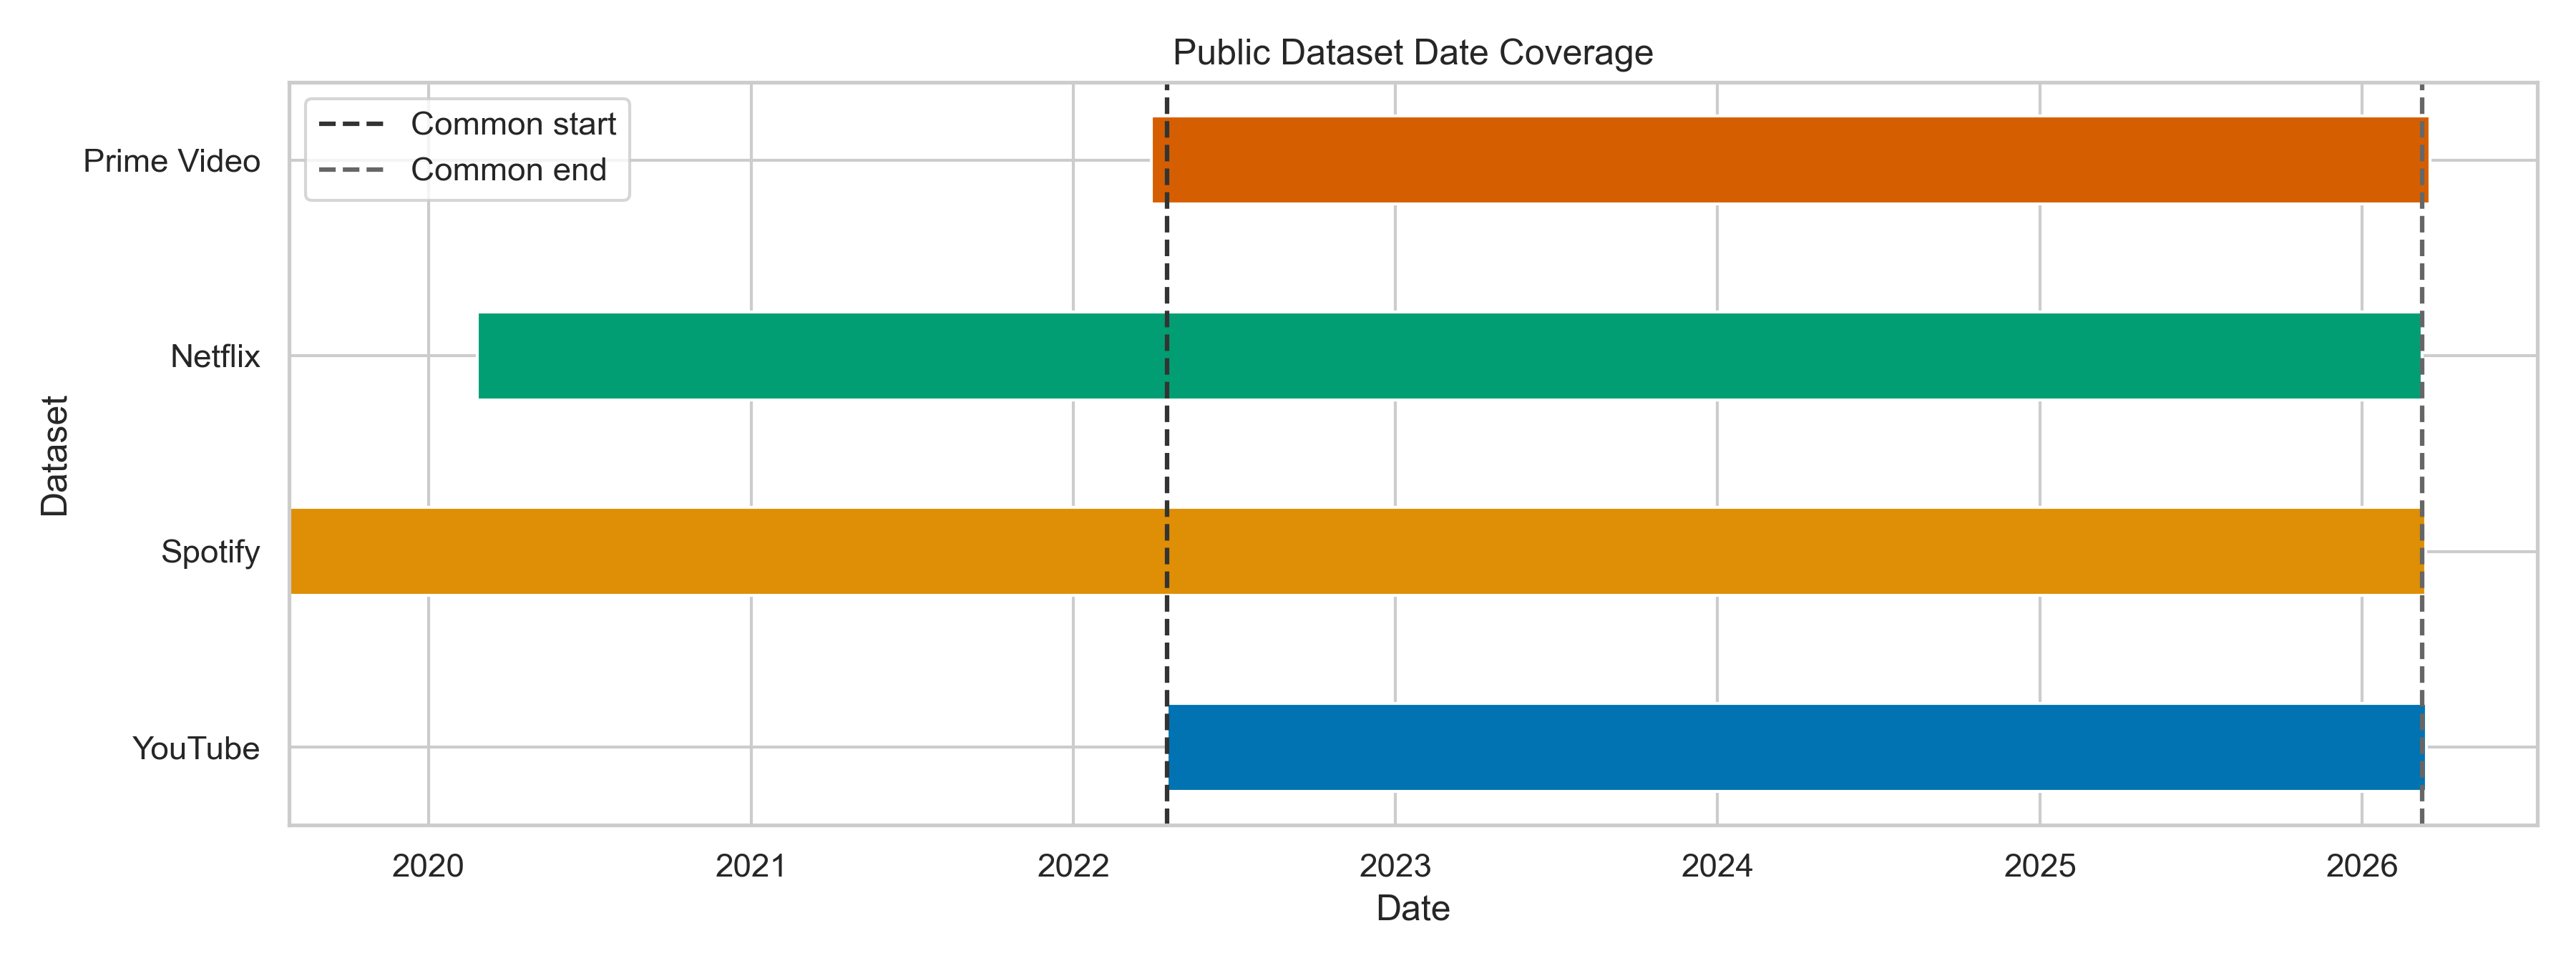
\includegraphics[width=0.86\textwidth]{../EDA/combined_images/combined_dataset_date_coverage.png}
\caption{Dataset date coverage. The common comparison window is 2022-04-17 to 2026-03-10.}
\label{fig:coverage}
\end{figure}

\begin{figure}[H]
\centering
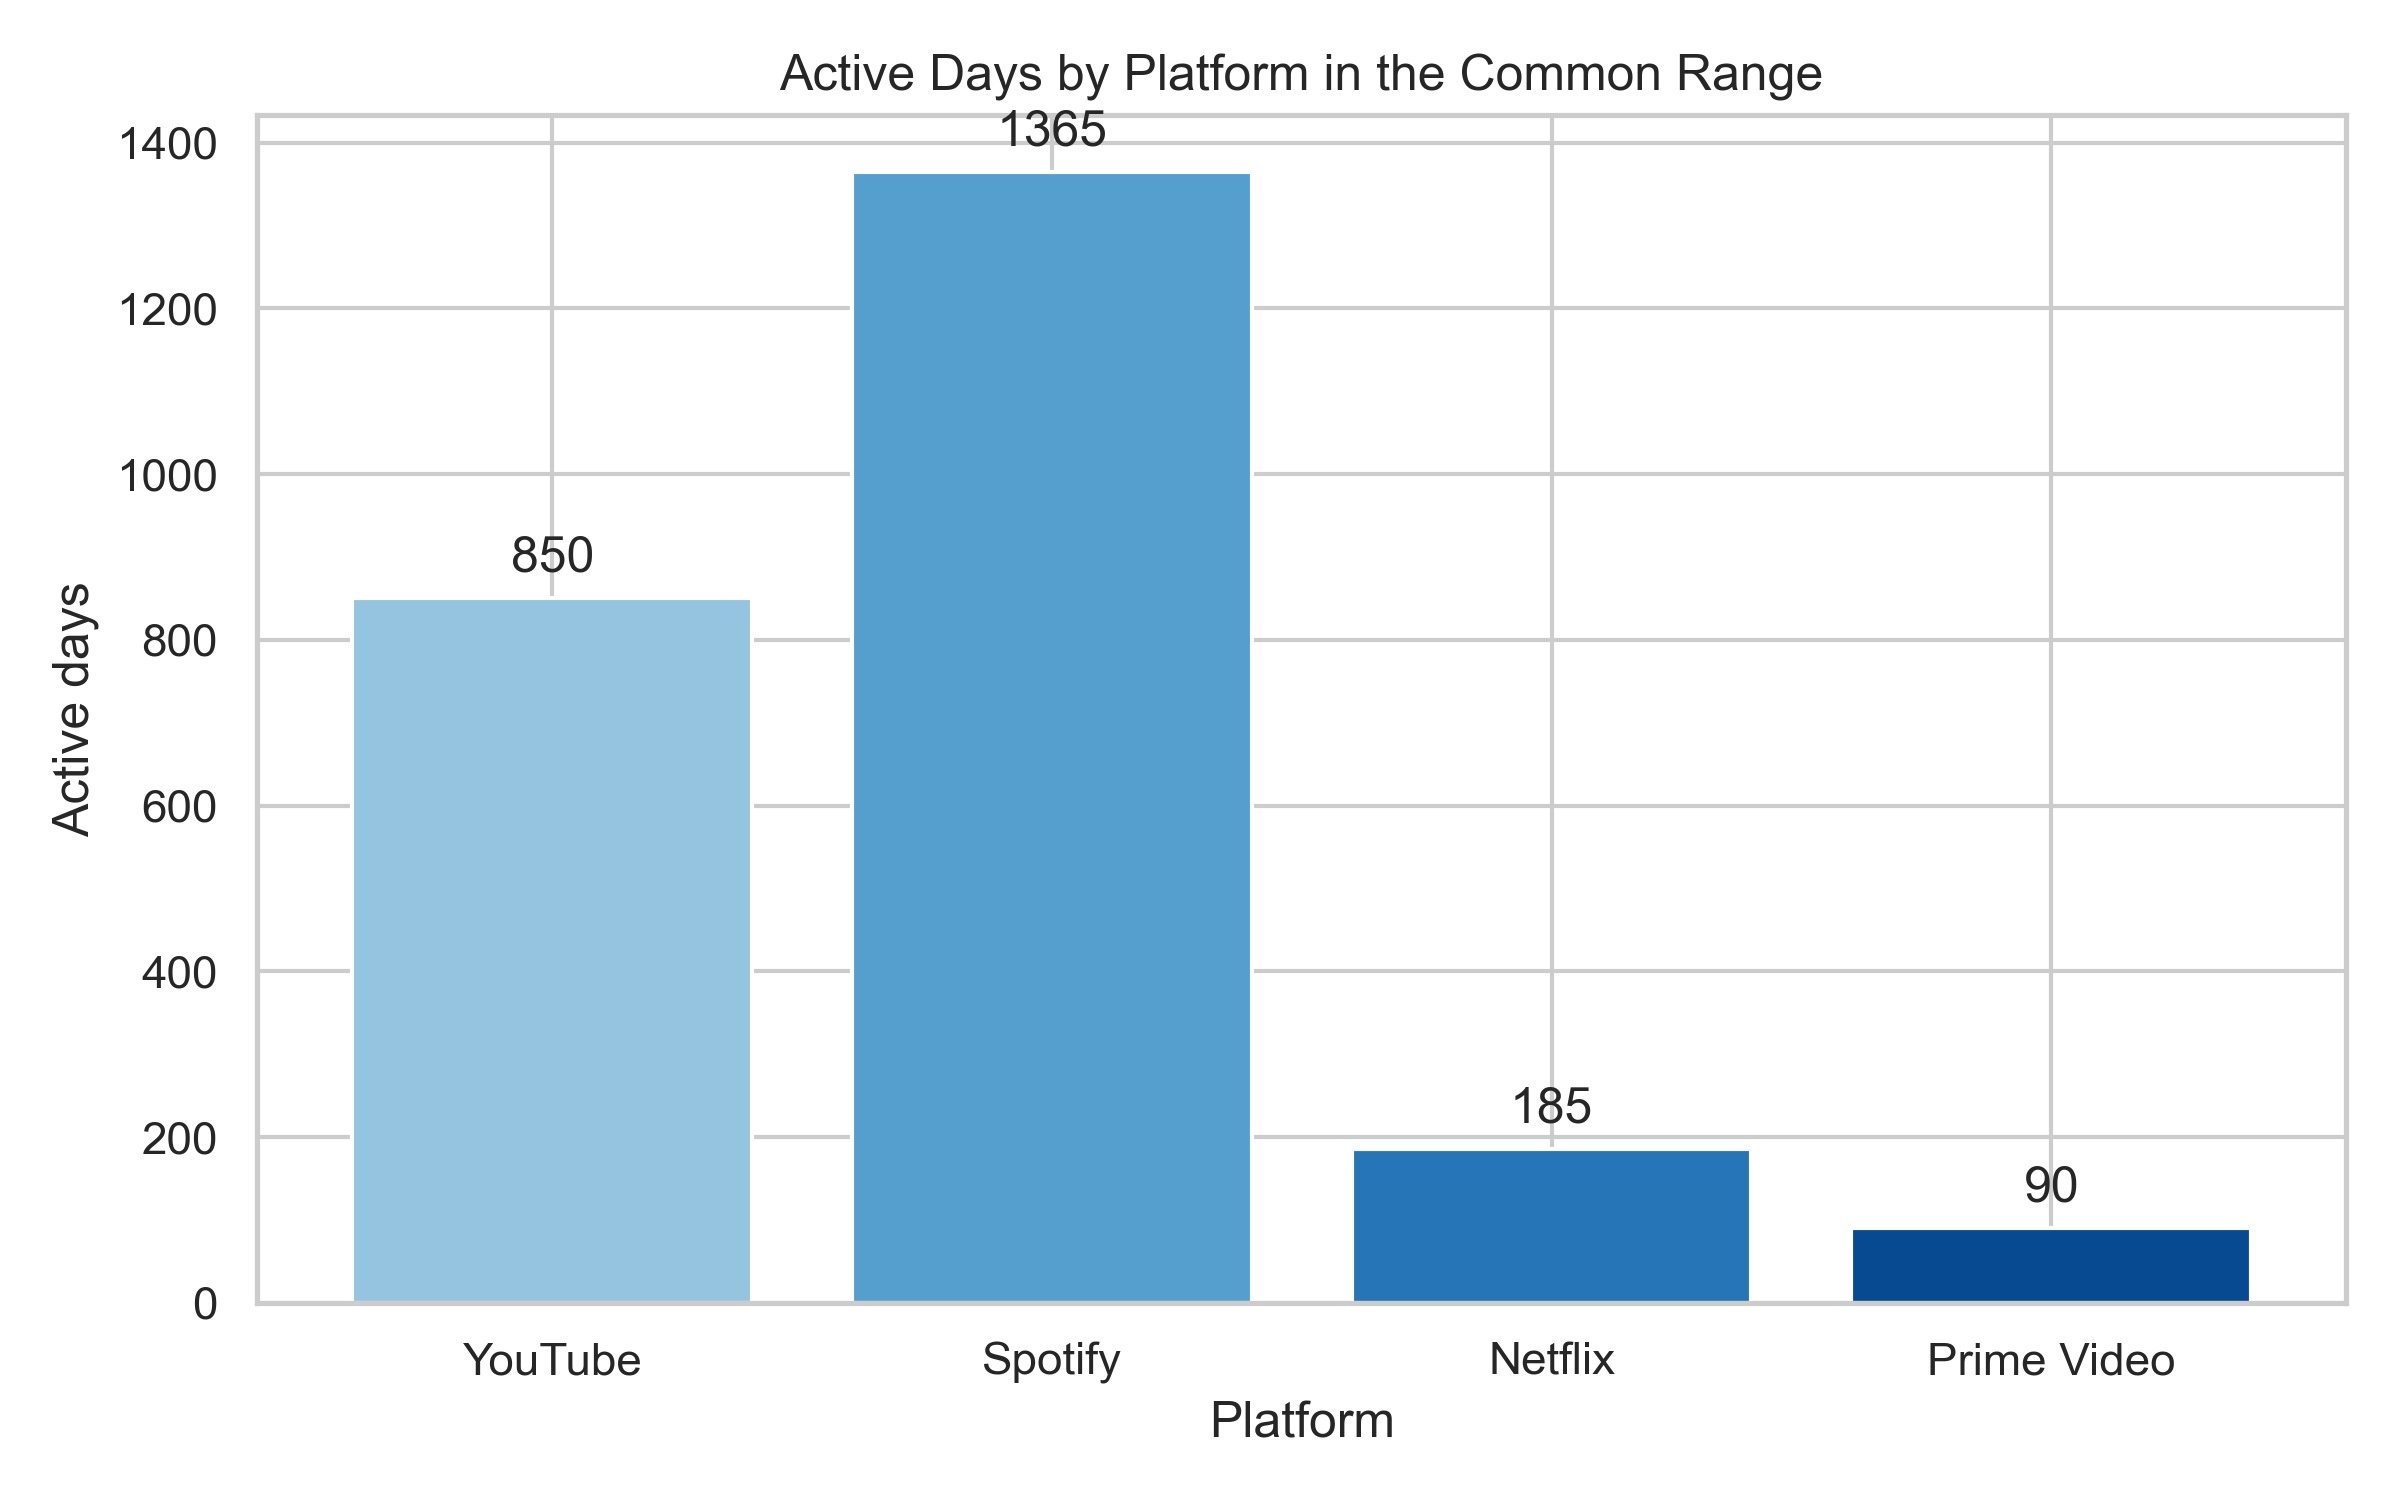
\includegraphics[width=0.86\textwidth]{../EDA/combined_images/combined_active_days_by_platform.png}
\caption{Active days by platform in the common range. This figure explains why some platform comparisons are sparse.}
\label{fig:active-days}
\end{figure}

The combined plots also helped shape the hypothesis choices. \figref{fig:combined-trends} shows that each platform has its own timing and scale. \figref{fig:corr} shows that platform variables are not all strongly related to each other, and \figref{fig:after2130} is directly connected to the late-evening hypothesis.

\begin{figure}[H]
\centering
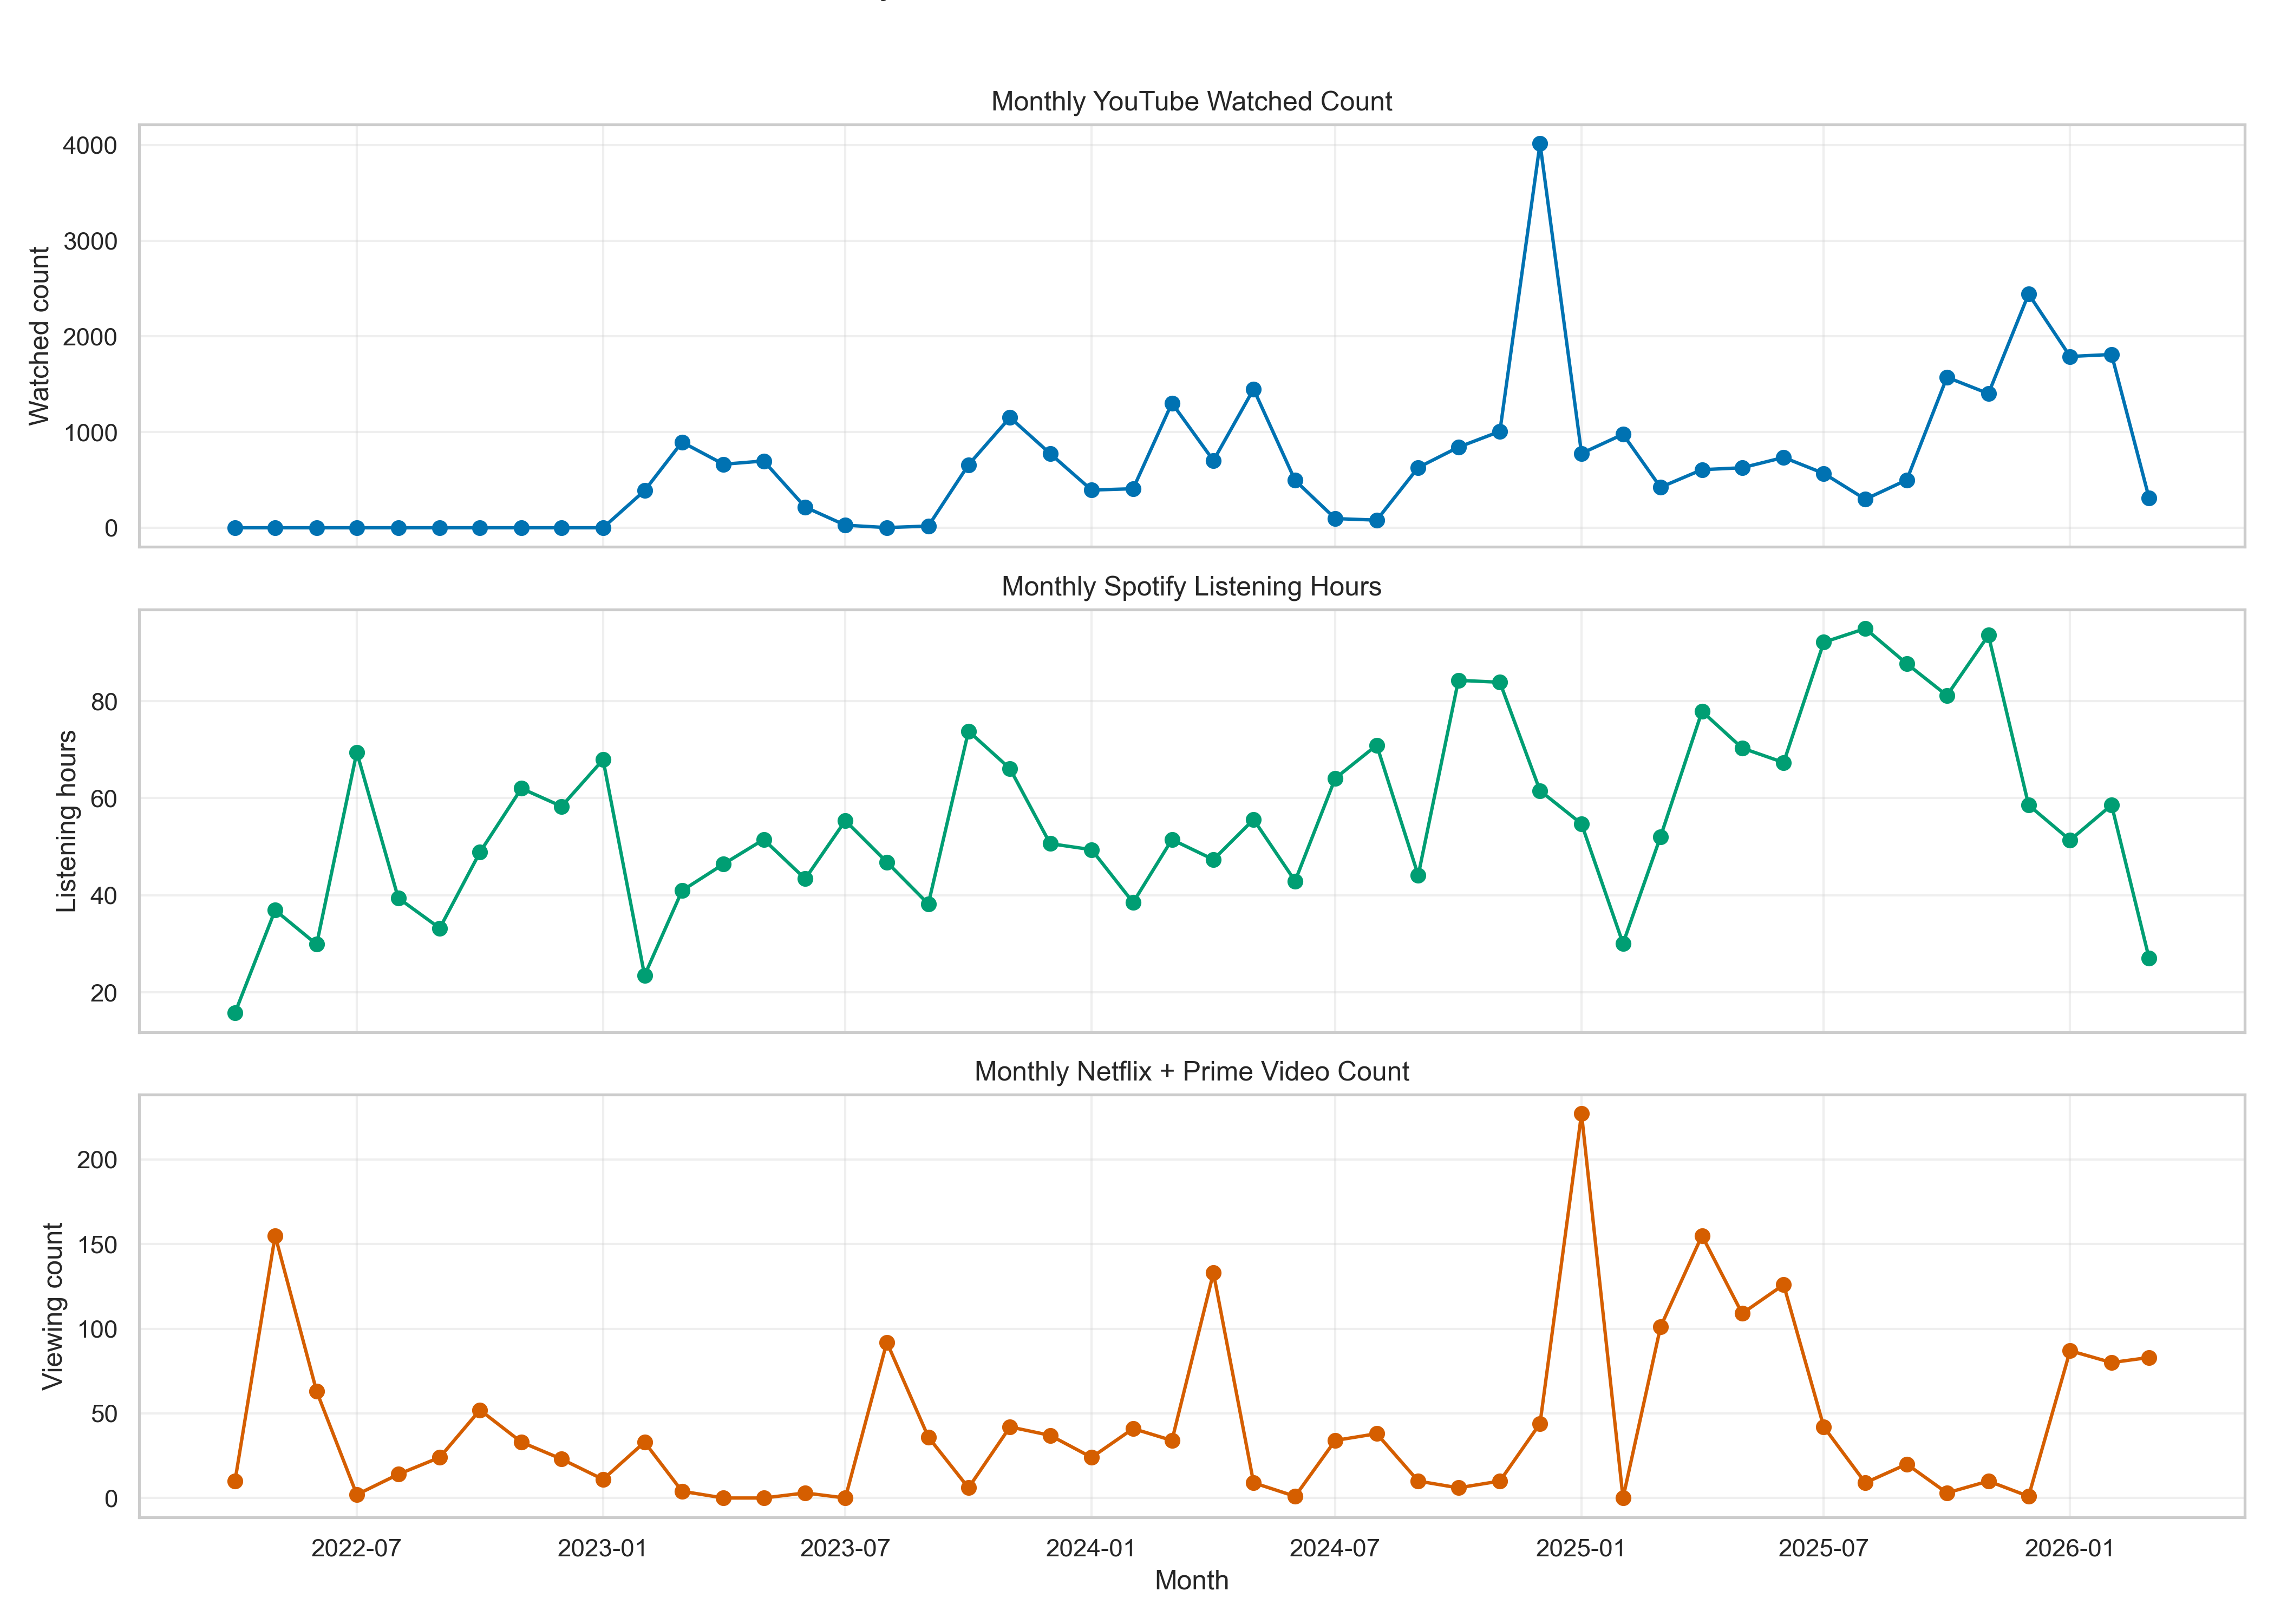
\includegraphics[width=0.86\textwidth]{../EDA/combined_images/combined_monthly_cross_platform_trends.png}
\caption{Monthly cross-platform trends. The panels are separated because platform units differ.}
\label{fig:combined-trends}
\end{figure}

\begin{figure}[H]
\centering
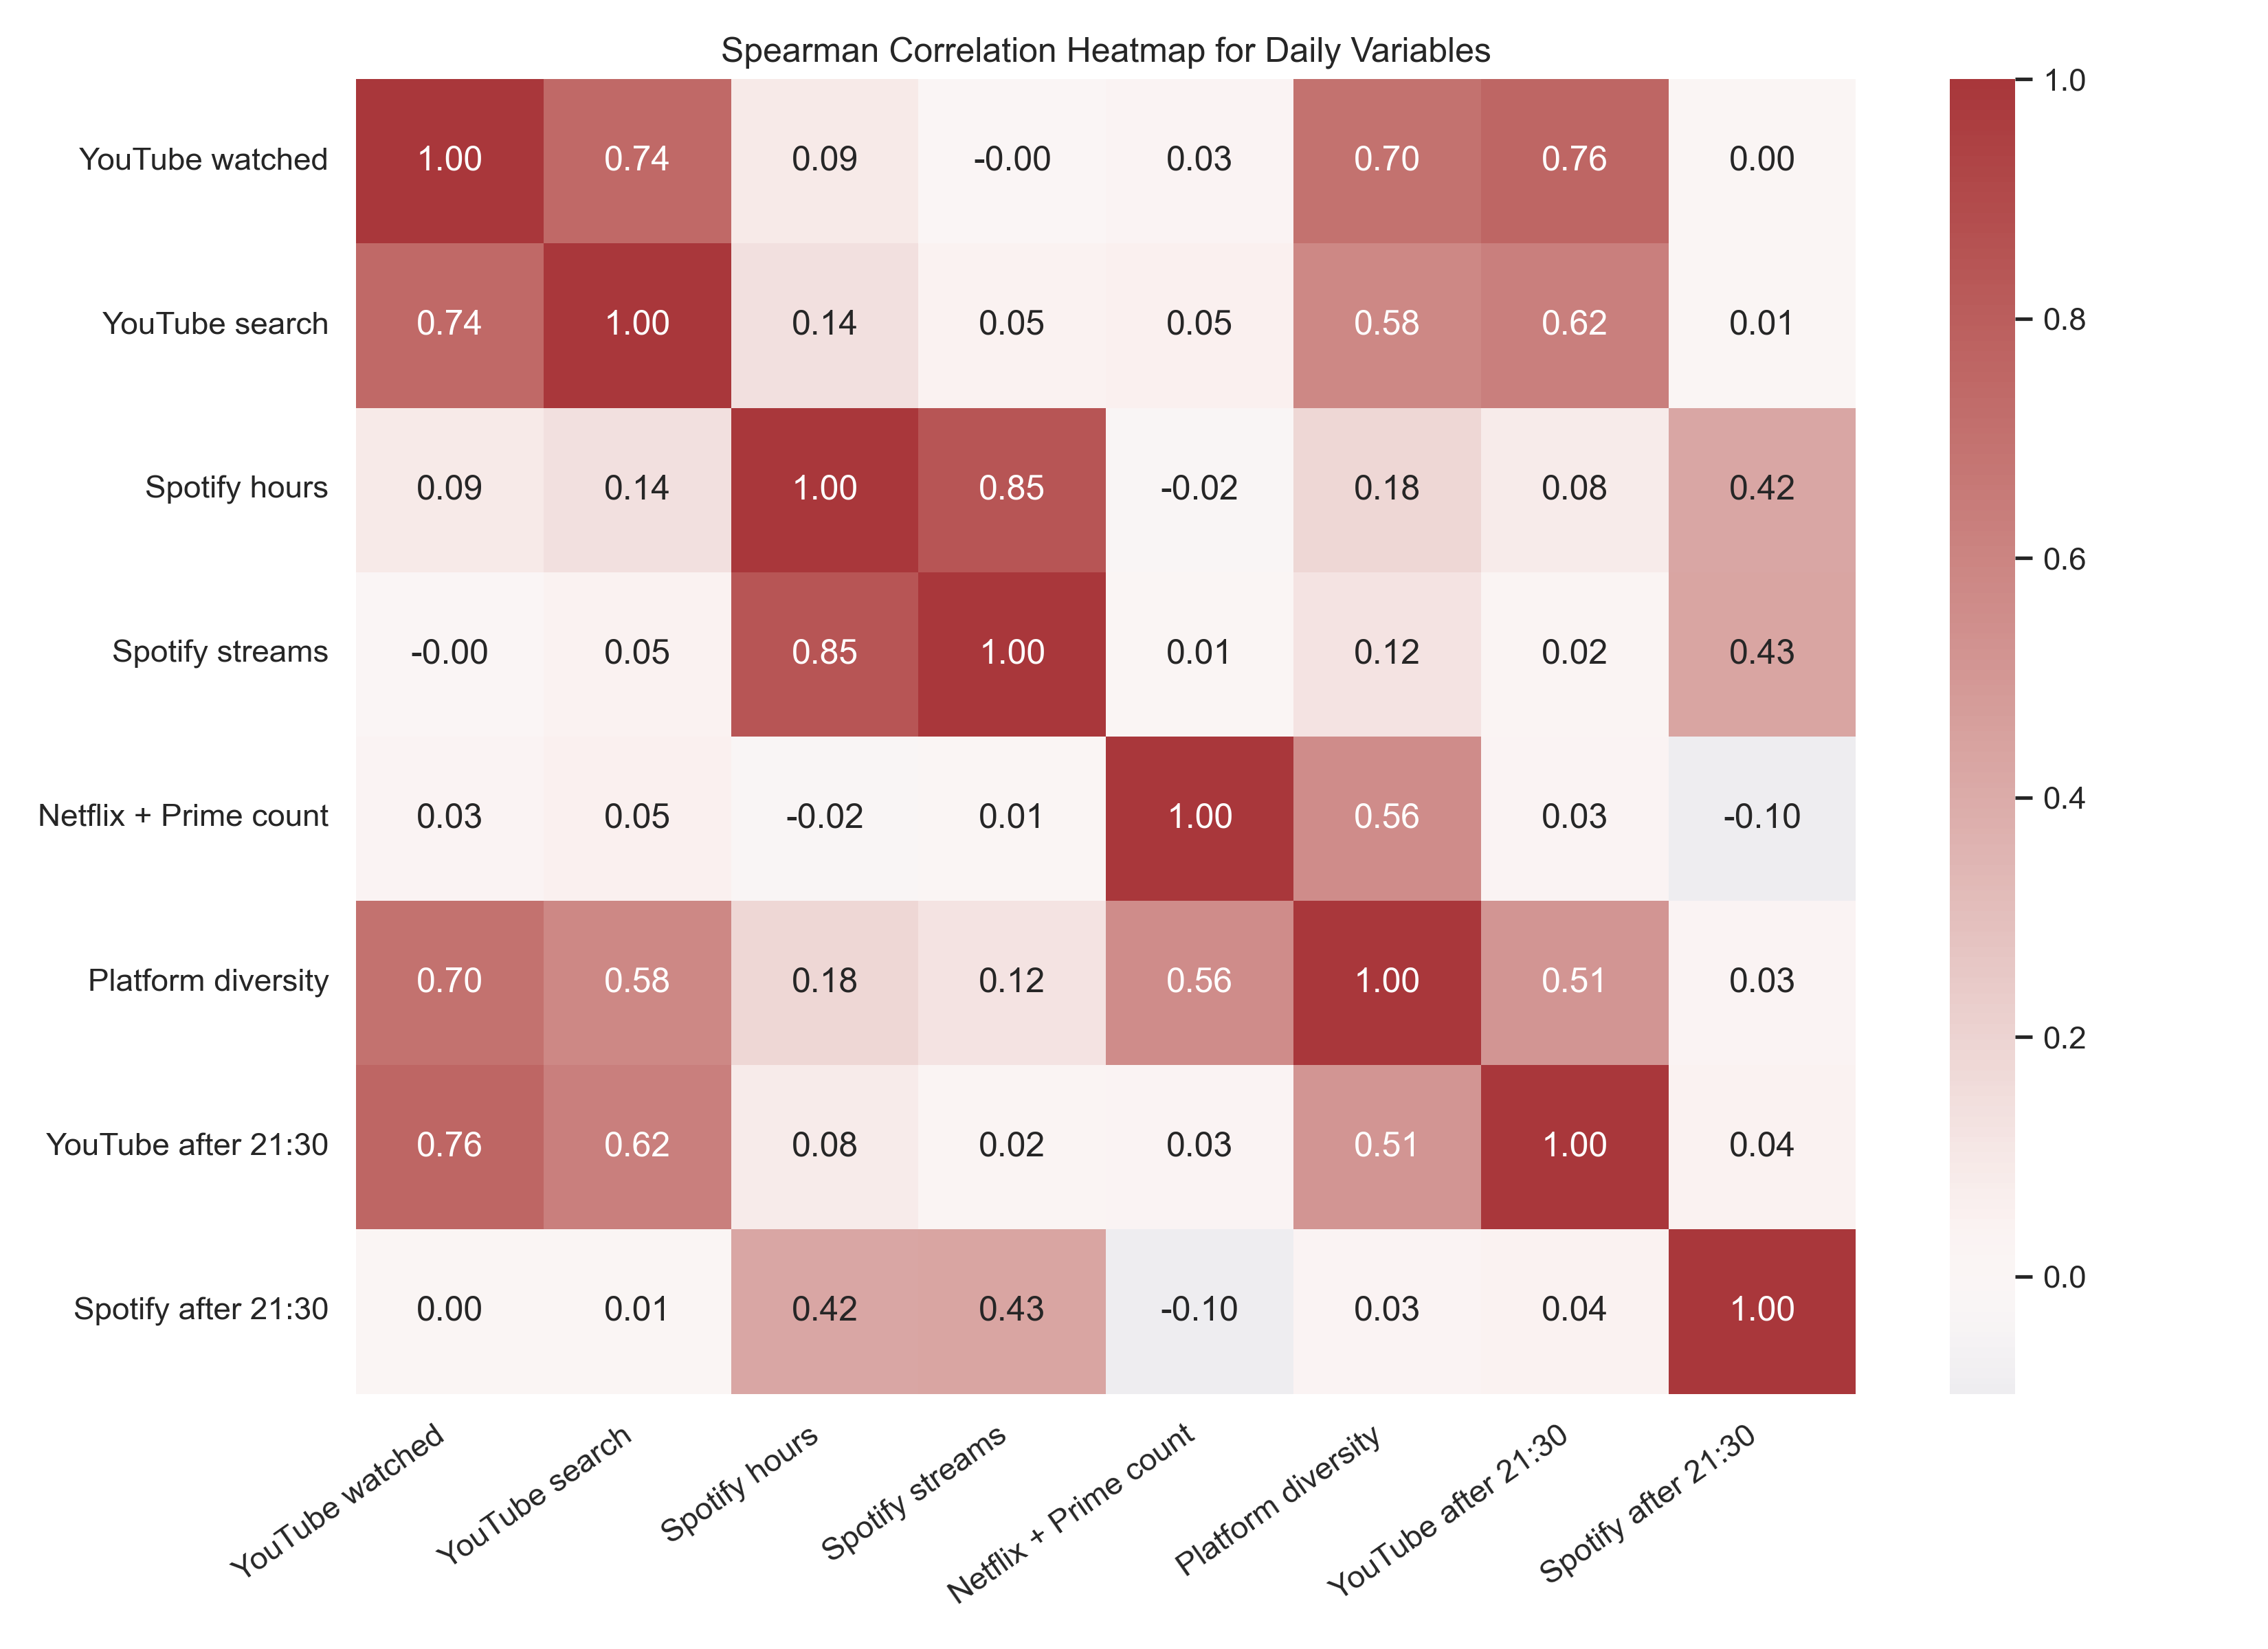
\includegraphics[width=0.86\textwidth]{../EDA/combined_images/combined_daily_variable_correlation_heatmap.png}
\caption{Daily-variable correlation heatmap. This figure was useful for checking same-day relationships before hypothesis testing.}
\label{fig:corr}
\end{figure}

\begin{figure}[H]
\centering
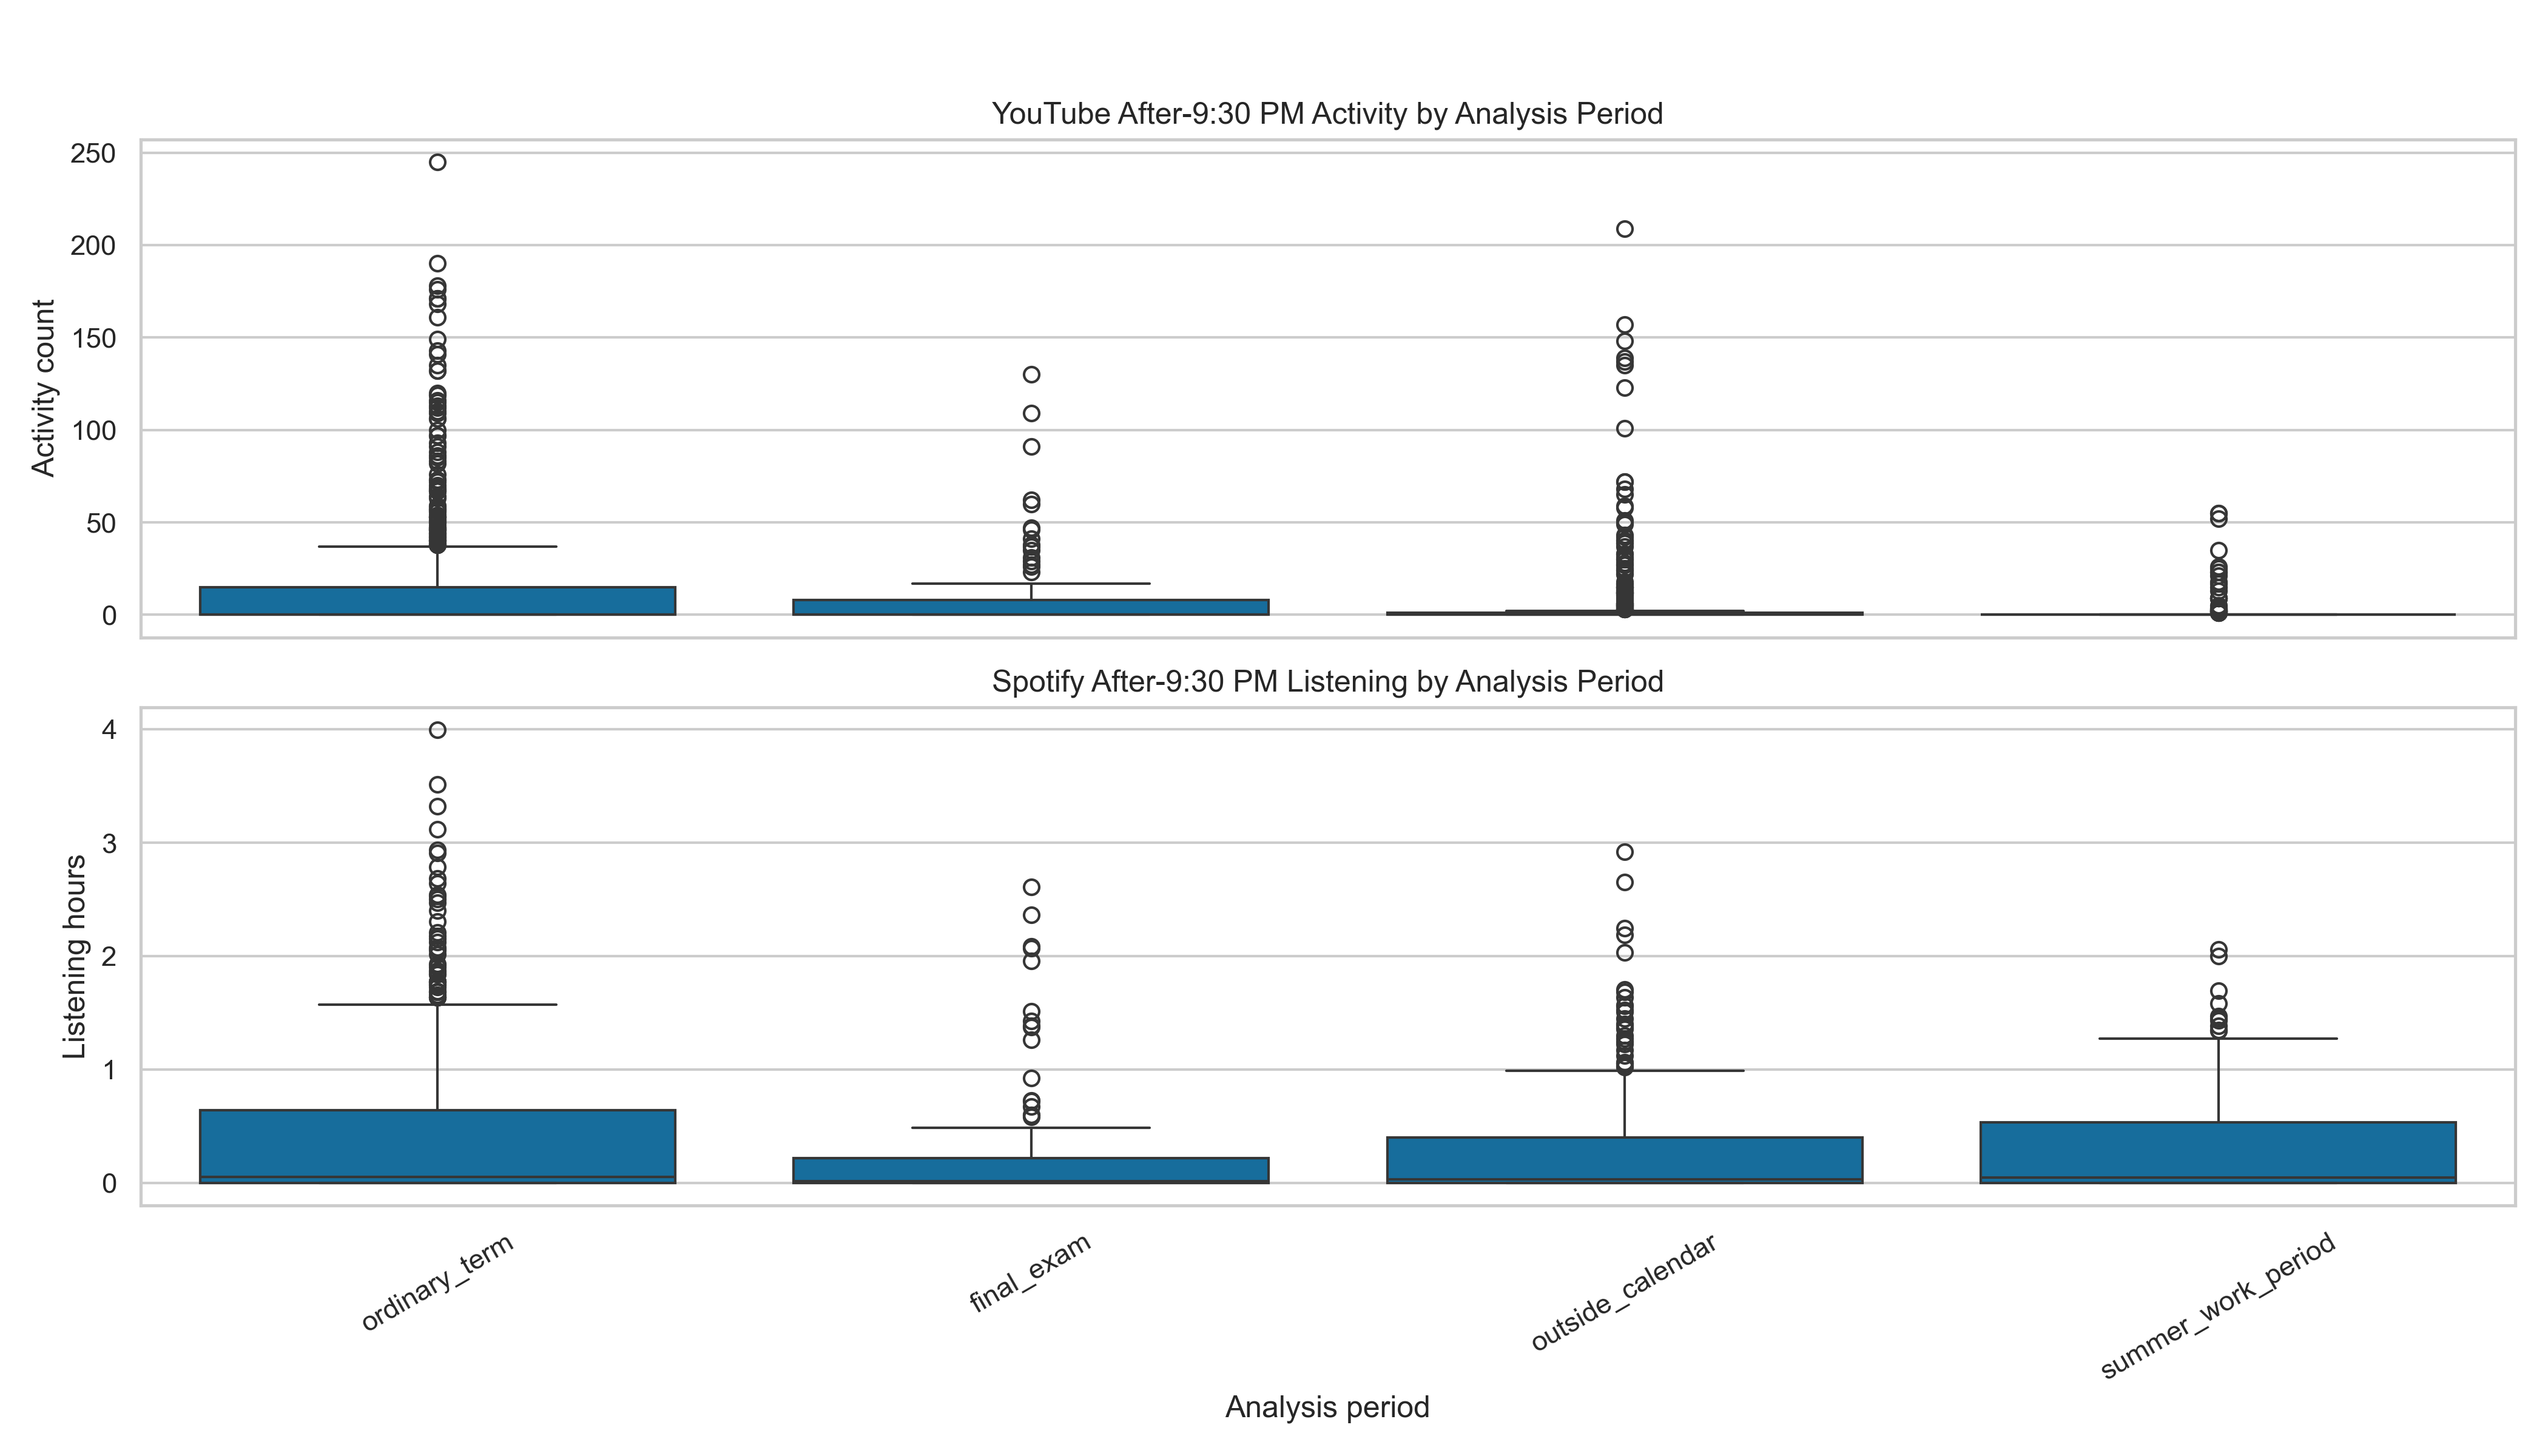
\includegraphics[width=0.86\textwidth]{../EDA/combined_images/combined_after_2130_by_analysis_period_boxplots.png}
\caption{After-21:30 activity by analysis period. This is directly related to the late-evening entertainment hypothesis.}
\label{fig:after2130}
\end{figure}

\section*{Hypotheses and Testing Method}
The formal hypothesis tests use the combined daily panel. For final-exam comparisons, I only compared \texttt{final\_exam} and \texttt{ordinary\_term}. Outside-calendar and summer-work days were kept for descriptive context but not included in the formal final-versus-ordinary tests.

Because the daily variables are skewed and often zero-heavy, I used one-sided Mann--Whitney U tests for the final-exam comparisons. This test does not assume normally distributed daily activity values, which is more appropriate for this dataset than a standard t-test. For the same-day Spotify and YouTube co-usage hypothesis, I used a one-sided Spearman correlation because it checks monotonic rank association rather than assuming a linear relationship.

For the first hypothesis, the question was broad: ``Does entertainment usage decrease during finals?'' Since the platforms have different units, I did not combine them into one artificial score. Instead, I tested the hypothesis separately for YouTube watched count, Spotify listening hours, Netflix viewing count, and Prime Video viewing count.

\begin{table}[H]
\centering
\scriptsize
\caption{Hypotheses used in the current testing stage.}
\label{tab:hypotheses}
\begin{tabularx}{\textwidth}{p{0.17\textwidth} X X p{0.19\textwidth}}
\toprule
\textbf{Hypothesis} & \textbf{Null hypothesis (H0)} & \textbf{Alternative hypothesis (H1)} & \textbf{Method}\\
\midrule
H1: Entertainment usage during academic pressure & Platform activity does not differ between final-exam days and ordinary-term days. & Final-exam days have lower platform activity. & One-sided Mann--Whitney U, tested separately by platform.\\
H2: Platform diversity during academic pressure & Platform diversity does not differ between final-exam days and ordinary-term days. & Platform diversity is lower during finals. & One-sided Mann--Whitney U.\\
H3: Netflix + Prime and YouTube activity & YouTube watched count does not differ between Netflix + Prime active and inactive days. & YouTube watched count is lower on Netflix + Prime active days. & One-sided Mann--Whitney U.\\
H4: Spotify and YouTube co-usage & Spotify hours are not associated with YouTube watched count. & Spotify hours are positively associated with YouTube watched count. & One-sided Spearman correlation.\\
H5: After-9:30 PM entertainment during finals & Late-evening entertainment share does not differ between final-exam days and ordinary-term days. & Late-evening share is lower during finals. & One-sided Mann--Whitney U, tested separately for YouTube and Spotify.\\
\bottomrule
\end{tabularx}
\end{table}

\section*{Hypothesis Test Results}
Table~\ref{tab:results} gives the current raw p-value results. The significance level was set to $\alpha=0.05$. These are still basic results because multiple tests are being run, so the p-values should be interpreted cautiously. \figref{fig:hypothesis-visual} visualizes the same result pattern and makes it easier to see which tests are below the 0.05 threshold.

\begin{table}[H]
\centering
\scriptsize
\caption{Current hypothesis test results.}
\label{tab:results}
\begin{tabularx}{\textwidth}{p{0.08\textwidth} p{0.26\textwidth} p{0.17\textwidth} r X}
\toprule
\textbf{Hyp.} & \textbf{Outcome} & \textbf{Decision} & \textbf{Raw p-value} & \textbf{Interpretation}\\
\midrule
H1 & YouTube watched count & Do not reject H0 & 0.0908 & YouTube watched count was lower in finals on average, but not enough to reject H0.\\
H1 & Spotify listening hours & Do not reject H0 & 0.0697 & Spotify hours were lower in finals on average, but not enough to reject H0.\\
H1 & Netflix viewing count & Do not reject H0 & 0.8512 & Netflix did not support the expected lower-finals direction.\\
H1 & Prime Video viewing count & Do not reject H0 & 0.3890 & Prime Video did not provide enough evidence for lower finals usage.\\
H2 & Distinct active entertainment platforms & Do not reject H0 & 0.1305 & Platform diversity did not significantly decrease during finals.\\
H3 & YouTube watched count on Netflix + Prime active days & Do not reject H0 & 0.8731 & Long-form active days did not support lower YouTube watch activity.\\
H4 & Spotify hours and YouTube watched count & Reject H0 & 0.0002 & There is a statistically detectable but weak positive same-day association.\\
H5 & YouTube after-21:30 activity share & Reject H0 & 0.0059 & YouTube late-evening share was lower during finals.\\
H5 & Spotify after-21:30 listening-hour share & Reject H0 & 0.0361 & Spotify late-evening listening share was lower during finals.\\
\bottomrule
\end{tabularx}
\end{table}

\begin{figure}[H]
\centering
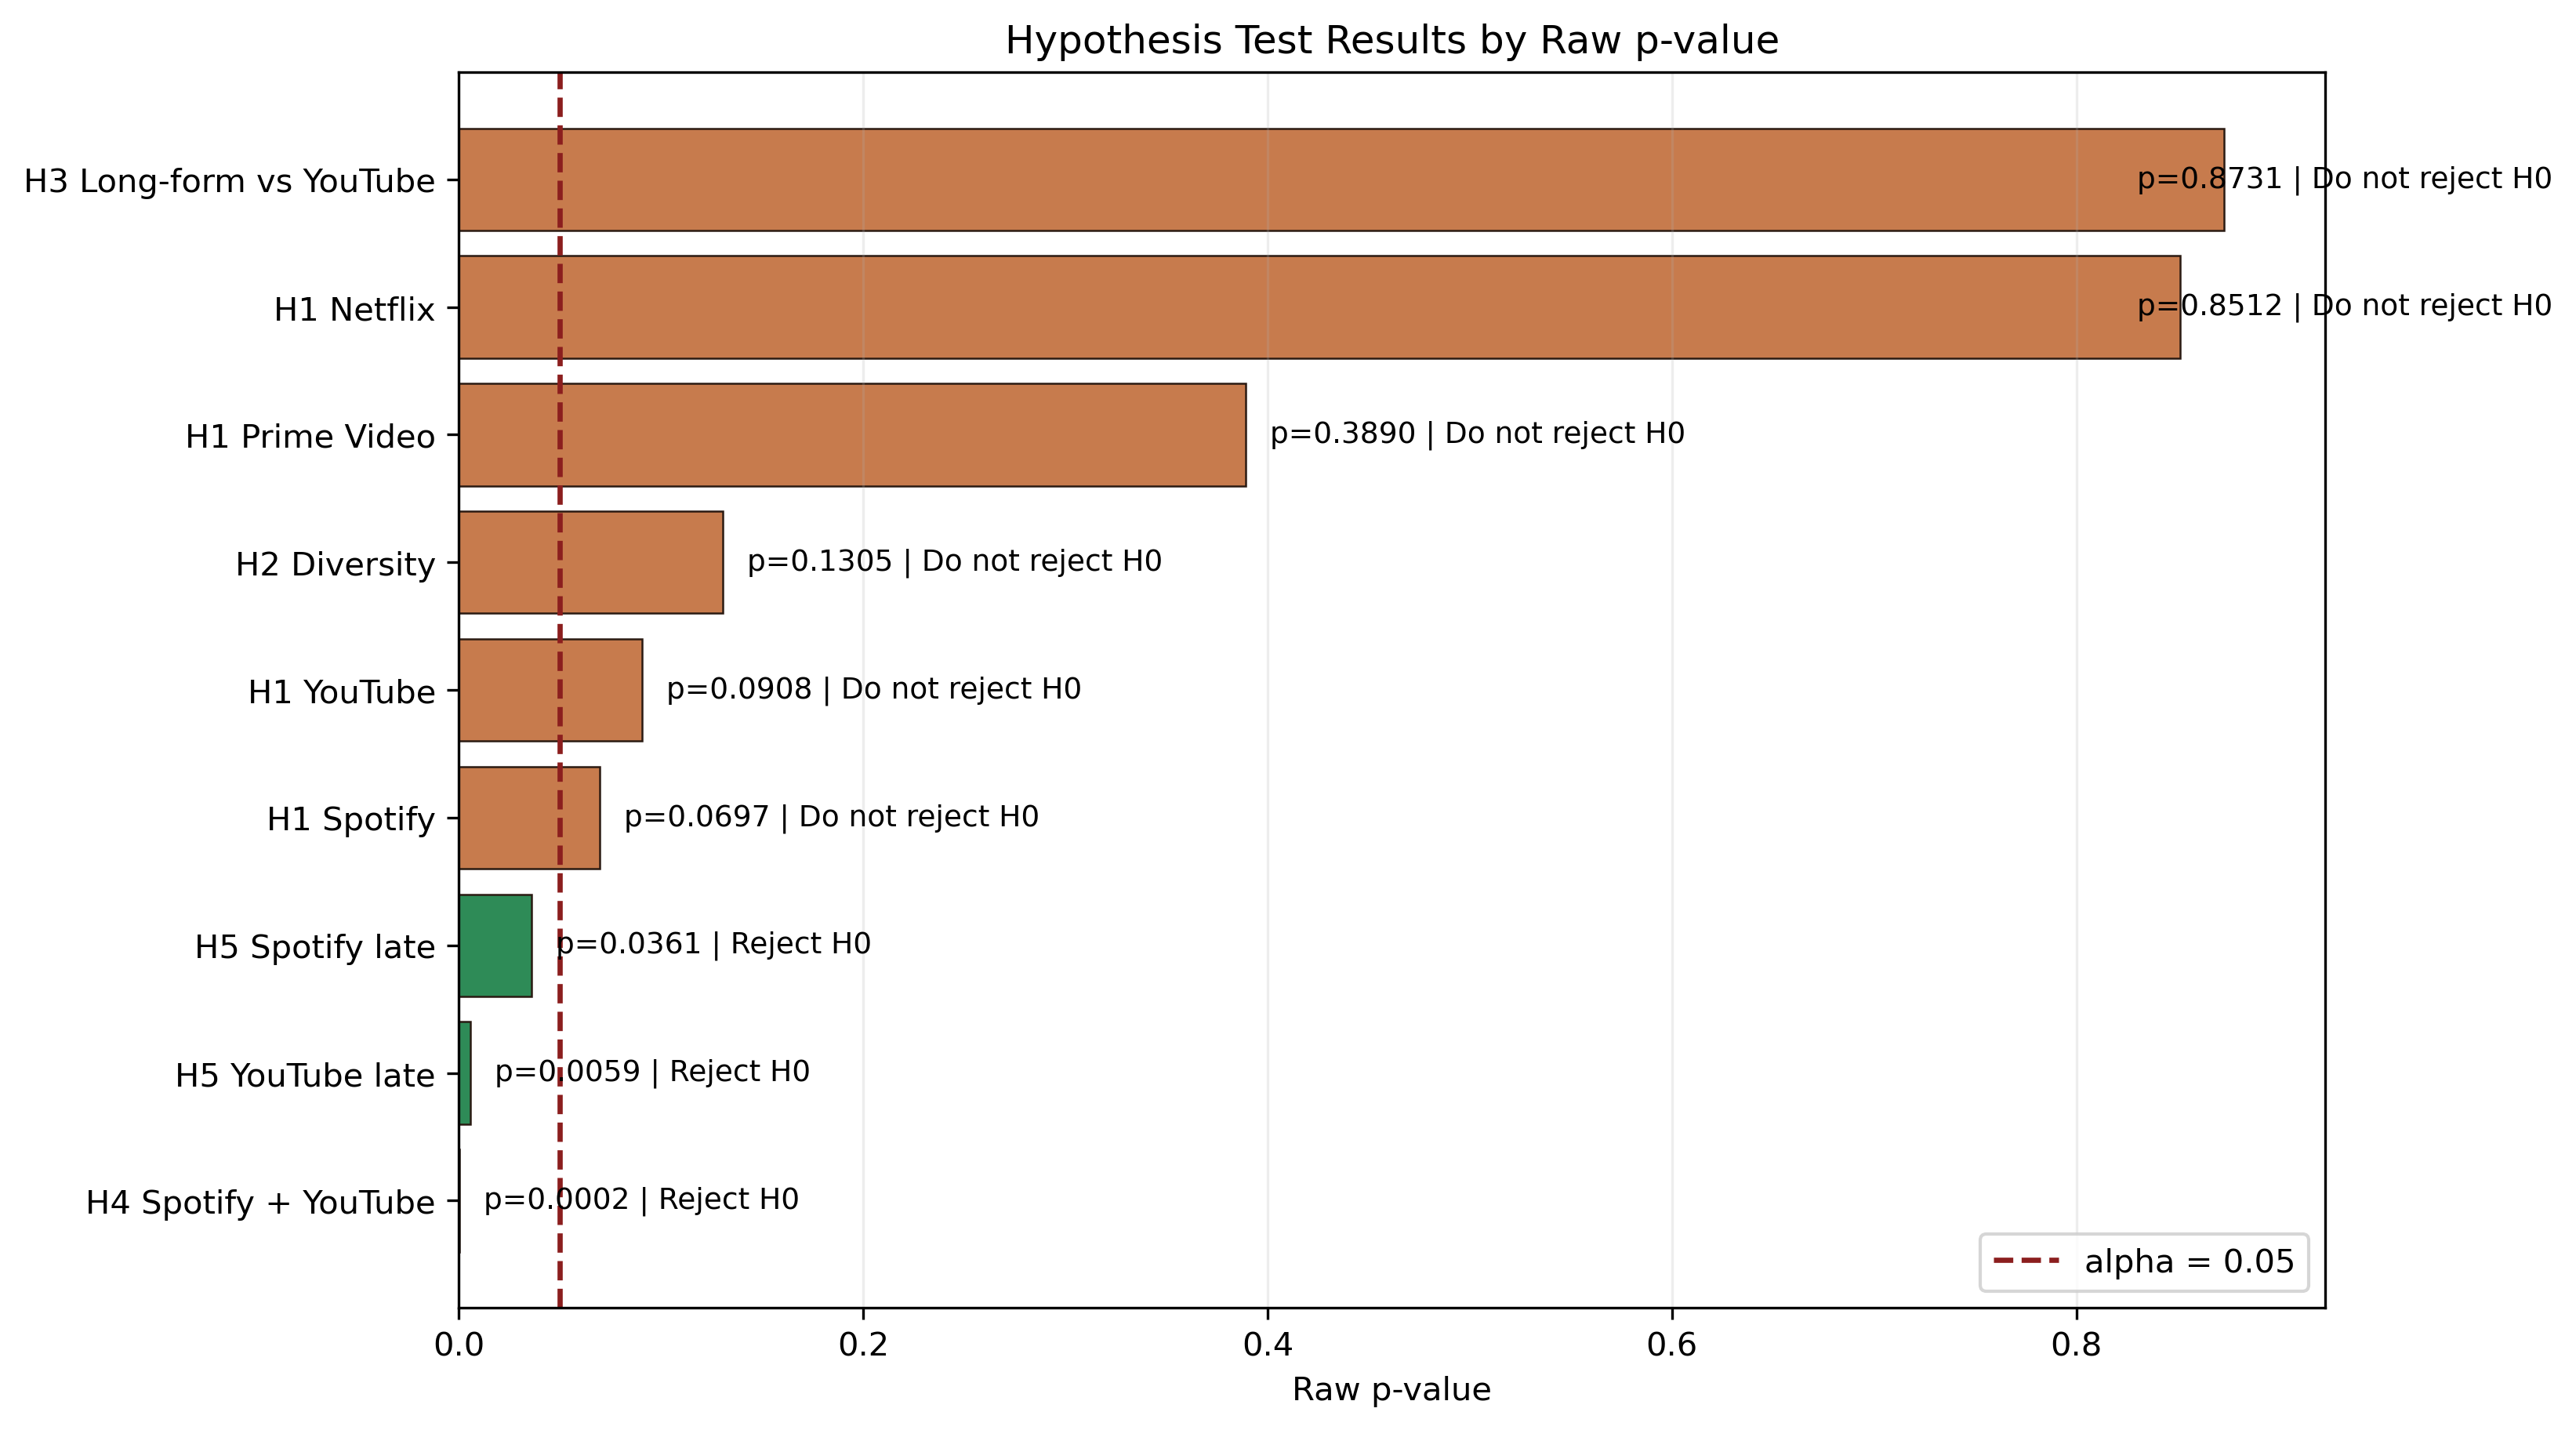
\includegraphics[width=0.92\textwidth]{../Hypothesis_Testing/hypothesis_results_decision_plot.png}
\caption{Hypothesis test results visualized by raw p-value. The dashed line marks $\alpha=0.05$.}
\label{fig:hypothesis-visual}
\end{figure}

The main result at this stage is that the broad entertainment-usage hypothesis was not supported strongly enough when tested platform by platform. However, late-evening activity during finals did show statistically significant lower shares for both YouTube and Spotify. The Spotify--YouTube co-usage hypothesis was also rejected, but the effect should be described as weak even though the p-value is small. This distinction is important because statistical detectability does not automatically mean a large practical effect.

\section*{Limitations and Next Steps}
There are several limitations at this stage. First, the datasets have different levels of temporal detail. Spotify and YouTube have exact timestamps, while Netflix and Prime Video are mostly date-level viewing records. Second, long-form streaming is sparse: many dates have zero Netflix and Prime Video activity. Third, the current hypothesis results use raw p-values, so multiple-testing correction should be considered later. Finally, YouTube watch time is only estimated from gaps between consecutive watch events, so it should be treated as an exploratory proxy rather than exact screen time.

The next stage of the project will focus on improving the analysis and preparing for the machine learning stage. A reasonable next step is to build derived daily features, such as lagged activity, rolling activity windows, academic-period labels, and simple platform-mix features. Any machine learning model should be evaluated carefully because this is a personal behavioral dataset with time dependence and uneven platform coverage.

\section*{AI Assistance Disclosure}
AI assistance was used for debugging, coding, and creating LaTeX style from normal text documents.

\clearpage
\appendix
\twocolumn[
\section*{Appendix: Additional EDA Figures}
The main body includes the figures most directly related to the current hypotheses and dataset structure. The remaining EDA figures are embedded below in two columns for compact review.
\vspace{0.8em}
]

\subsection*{YouTube EDA Figures}
\appendixfig{../EDA/youtube_images/youtube_activity_count_by_hour.png}{YouTube activity count by hour}
\appendixfig{../EDA/youtube_images/youtube_activity_count_by_target_kind.png}{YouTube activity count by target kind}
\appendixfig{../EDA/youtube_images/youtube_daily_after_2130_watched_count.png}{YouTube after-21:30 watched count}
\appendixfig{../EDA/youtube_images/youtube_daily_watched_and_search_counts.png}{Daily YouTube watched and search counts}
\appendixfig{../EDA/youtube_images/youtube_daily_watched_by_weekday_boxplot.png}{YouTube watched count by weekday}
\appendixfig{../EDA/youtube_images/youtube_daily_watched_search_distribution.png}{YouTube watched/search distribution}
\appendixfig{../EDA/youtube_images/youtube_daily_watched_vs_search_scatter.png}{YouTube watched versus search scatter}
\appendixfig{../EDA/youtube_images/youtube_eda_overview_panel.png}{YouTube EDA overview panel}
\appendixfig{../EDA/youtube_images/youtube_monthly_after_2130_share.png}{Monthly YouTube after-21:30 share}
\appendixfig{../EDA/youtube_images/youtube_top_masked_channel_refs.png}{Top masked YouTube channel references}

\subsection*{Spotify EDA Figures}
\appendixfig{../EDA/spotify_images/spotify_daily_after_2130_hours.png}{Spotify after-21:30 listening hours}
\appendixfig{../EDA/spotify_images/spotify_daily_hours_by_weekday_boxplot.png}{Spotify daily hours by weekday}
\appendixfig{../EDA/spotify_images/spotify_daily_hours_distribution.png}{Spotify daily hours distribution}
\appendixfig{../EDA/spotify_images/spotify_daily_listening_hours.png}{Spotify daily listening hours}
\appendixfig{../EDA/spotify_images/spotify_eda_overview_panel.png}{Spotify EDA overview panel}
\appendixfig{../EDA/spotify_images/spotify_listening_hours_by_hour.png}{Spotify listening hours by hour}
\appendixfig{../EDA/spotify_images/spotify_top_15_artists_by_hours.png}{Top Spotify artists by hours}
\appendixfig{../EDA/spotify_images/spotify_top_15_tracks_by_hours.png}{Top Spotify tracks by hours}

\subsection*{Netflix and Prime Video EDA Figures}
\appendixfig{../EDA/prime_netflix_images/combined_long_form_distribution.png}{Combined long-form distribution}
\appendixfig{../EDA/prime_netflix_images/combined_long_form_streaming_daily_count.png}{Combined long-form daily count}
\appendixfig{../EDA/prime_netflix_images/daily_count_distribution_active_days.png}{Daily count distribution on active days}
\appendixfig{../EDA/prime_netflix_images/daily_viewing_count_netflix_vs_prime.png}{Daily viewing count: Netflix versus Prime Video}
\appendixfig{../EDA/prime_netflix_images/long_form_daily_count_by_weekday_boxplot.png}{Long-form daily count by weekday}
\appendixfig{../EDA/prime_netflix_images/long_form_streaming_by_platform.png}{Long-form streaming by platform}
\appendixfig{../EDA/prime_netflix_images/monthly_long_form_count_by_platform.png}{Monthly long-form count by platform}
\appendixfig{../EDA/prime_netflix_images/netflix_title_quality_split.png}{Netflix title quality split}
\appendixfig{../EDA/prime_netflix_images/netflix_vs_prime_daily_scatter.png}{Netflix versus Prime daily scatter}
\appendixfig{../EDA/prime_netflix_images/prime_netflix_eda_overview_panel.png}{Prime and Netflix EDA overview panel}
\appendixfig{../EDA/prime_netflix_images/prime_video_record_type_split.png}{Prime Video record type split}
\appendixfig{../EDA/prime_netflix_images/top_15_netflix_title_groups.png}{Top Netflix title groups}
\appendixfig{../EDA/prime_netflix_images/top_15_prime_video_title_groups.png}{Top Prime Video title groups}

\subsection*{Combined EDA Figures}
\appendixfig{../EDA/combined_images/combined_daily_distribution_overview.png}{Combined daily distribution overview}
\appendixfig{../EDA/combined_images/combined_eda_overview_panel.png}{Combined EDA overview panel}
\appendixfig{../EDA/combined_images/combined_monthly_after_2130_activity.png}{Combined monthly after-21:30 activity}
\appendixfig{../EDA/combined_images/combined_platform_activity_by_analysis_period_boxplots.png}{Combined platform activity by analysis period}
\appendixfig{../EDA/combined_images/combined_platform_diversity_by_analysis_period.png}{Combined platform diversity by analysis period}
\appendixfig{../EDA/combined_images/combined_relative_activity_by_analysis_period.png}{Combined relative activity by analysis period}

\end{document}
